
\chapter{AC Power}
\section{Power}

Recall that for DC:
\[
P = VI = I^2 R
\]

These are still true for AC, but now $P$ is a time function as well
that we can call $p(t)$, the instantaneous power.  It's units
are  Watts.

\subsection{Sign Convention for Power}

We need to {\bf define} ``positive'' and ``negative'' when we talk about
power. For example for a generator, positive power is power (energy) flowing
{\bf out} but for a speaker electrical power is the power (energy) flowing
{\bf in}!     This is just a convention however.  Most of the time we will declare:

\begin{quotation} ``Positive power means power dissipated (or converted) inside
a circuit.'' \end{quotation}

But then an unfortunate generator manufacturer would have to specify their
product as ``New
and improved model XY270 has -10kW output!'' which does not generate many sales.

So we need to understand the voltage and current sign conventions as follows

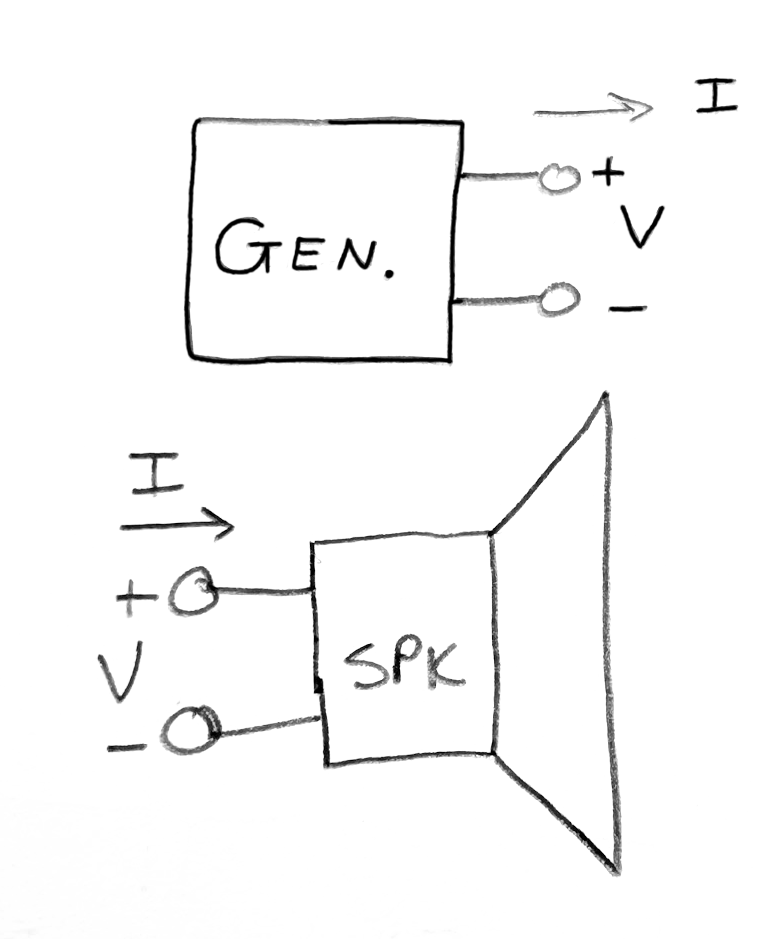
\includegraphics[width=0.3\textwidth]{figsChapt03/IE47318.png}

The $\pm$ indicates how we define positive voltage, and the direction arrow indicates
how we define positive current.

For the generator:
\[
P = VI = 1000V\times 10A = 10kW
\]
and for the speaker as shown:
\[
P = VI = 10V\times5A  =50W
\]
and everybody's happy.







\subsection{Power in the sinusoidal steady state}
Let's assume sinusoidal steady state and we have
\[
i(t) = I_M \cos(\omega t + \phi)
\]
\[
v(t) = V_M \cos(\omega t)
\]

\noindent We define the {\bf Average Power} as:
\[
P_{AV} = \frac{1}{T} \int_0^T i(t) v(t) \, dt
\]
where $T = \frac {\omega}  {2\pi}\;\; \text{the~period~of}  \;\; i(t), v(t) = \frac{2\pi}{\omega}$.


\noindent Note this is  also true of multiple periods,
\[
\int_0^{nT} dt \text{~~or~even} \int_{-\infty}^{-\infty}dt
\]



\noindent so,
\[
P_{AV_{\text{Sinusoid}}} = I_MV_M\frac{1}{T} \int_0^{2\pi/\omega}  \cos(\omega t + \phi) \cos(\omega t) dt
\]

\[
= I_M V_M \frac{\omega}{2\pi} \left[ \frac{\pi \cos(\phi)}{\omega} \right] \quad
\]
(We've looked up that integral in a table).   Finally we get:

\[
P_{AV_{\text{Sinusoid}}} = \frac{I_M V_M}{2} \cos(\phi)
\]
Where $ \phi = $ the angle between voltage and current.

Note that this is almost like the DC result, $P=IV$.   We
define the important quantity {\bf power factor}, as

\[
PF \equiv \cos(\phi)
\]
Power Factor is
a number between zero and 1 which depends on the phase angle between
voltage and current (note it's always positive for phase angles between
$\pm 90^\circ$.)


\subsection{Power in a General Impedance}

%\includegraphics[width=0.3\textwidth]{figsChapt03/SA65016.png}  %2-Oct-25
With reference to this simple circuit, we can write
%
% \[
% i(t) = I_M \cos(\omega t + \phi)
% \]
% \[
% \vec{V} = \vec{I} Z \Rightarrow v(t) = V_M \cos(\omega t + \phi + \angle z)
% \]
% \[
% (V_M = I_M |Z|)
% \]
% \[
% \alpha = \phi + \angle z
% \]

\[
p(t) = i(t) \cdot v(t)
\]
for the sinusoidal steady state, and defining $\phi=0$ according
to the phase angle of the applied voltage wave,
\[
v(t) = V_M\cos(\omega t)
\]
\[
i(t) = I_M\cos(\omega t + \phi)
\]
($V_M, I_M$ are real numbers)

\[
p(t) = v(t) \cdot i(t) = V_M I_M \cos(\omega t ) \cos(\omega t + \phi )
\]
(note that $\phi = \angle{Z}$)

\noindent A trig identity is the  product of cosines formula\footnote{See wikipedia trig indentities}:

\[
\cos(a) \cos(b) = \frac {1} {2} (\cos(a-b) + \cos(a+b))
\]
where $a=\omega t$ and $b=\omega t + \phi$.

So using that we get:

\[
p(t) = \frac{I_M V_M }{2} \cos(\omega t -\omega t - \phi) + \frac{I_M V_M}{2} \cos(\omega t + \omega t + \phi )
\]

\[
p(t) = \frac{I_M V_M }{2} \cos( \phi) + \frac{I_M V_M}{2} \cos(2\omega t + \phi )
\]
Note also that $\cos(-x) = \cos(x)$ and that $V$ and $I$ are related by
\[
\vec V = \vec I Z
\]
so $\phi = \angle {Z}$

Perhaps the  most useful form of the result is
\[
p(t) = \frac{I_M V_M }{2} \cos( \angle{Z}) + \frac{I_M V_M}{2} \cos(2\omega t + \angle{Z})
\]

This has two components.
{\bf 1)} The average power (a {\bf constant}, $\frac{V_M I_M}{2} \cos(\angle Z)$) and
{\bf 2)} a time varying power ($\frac{I_M V_M}{2} \cos(2\omega t   + \angle Z)$).

If we are using RMS values instead of the absolute magnitudes $V_M, I_M$,
we note
\[
\frac {V_MI_M}  {2} = |\vec V_R||\vec I_R| = V_R I_R
\]

so we also have
\[
p(t) = V_RI_R\cos(\angle{Z}) + V_RI_Rcos(2\omega+\angle{Z})
\]

\subsection{Computing Power Waveforms with Python}

\vspace{0.3in}
In the following, we will make some python computations of $v(t), p(t)$
with a fixed $i(t)$.   The color code will be:
\begin{center}
\begin{tabular}{l|l}\hline
black  &  Current \\
blue   &  Voltage \\
red    &  Instantaneous Power \\
\end{tabular}
\end{center}
The current will be the same in each case, e.g.
\[
i(t) = 1.0\cos(t) \;\; \text{Amps} \to  \vec I = 1.0 \angle 0^\circ
\]
The python code will simply compute $p(t)$ at each instant of time and plot it.

\begin{listing}
\begin{minted}{python}
import numpy as np
import matplotlib.pyplot as plt
#
#   Visualize sinusoidal voltage and current and power
#     for R, L, C
w = 1
C = 1
R = 2.0
L = 0.5
j = 0.0+1.0j

ZR = R
ZC = 1.0/(j*w*C)
ZL = j*w*L
# choose an element:
Z = ZC
# titlestr = 'Resistor'
titlestr = 'Capacitor'
# titlestr = 'Resistor'

phi = np.angle(Z)
T = np.linspace(0,5*np.pi/2, 50)
V = (1.0 + 0j) * np.e**(j*w*T)  # complex sinusoid voltage
I = V/Z
Vr = np.real(V)
Ir = np.real(I)
P = Vr*Ir
i=0
for t in T:
   print(t, Vr[i], Ir[i], P[i])
fig = plt.figure(figsize=(10,10))
ax = plt.gca()
data = [Ir, Vr, P]
colors=['k','b','r']
for i in range(3):
    plt.plot(T,data[i], color=colors[i])
pi = np.pi
tickpts = np.array(range(12))
tickvals = pi/4 * tickpts
ax.set_xticks(tickvals)
ax.set_xlabel('wt (rad)')
ax.set_ylabel('Amplitude')
ax.legend(['Current', 'Voltage', 'Inst. Pwr.'])
plt.title('Voltage, Current, Power: '+titlestr)
plt.grid()
plt.show()
\end{minted}
\caption{Python Code for visualizing power waveforms (red).}
\label{lst:basicTustin}
\end{listing}


\paragraph{Capacitor}
Consider a capacitor where
\[
Z = \frac{j}{\omega C}, \quad V_M = I_M |Z| = \frac{I_M}{\omega C}, \quad \angle z = -\pi/2
\]

and again we assume sinusoidal steady state with
\[
v(t) = V_M \cos(\omega t)
\]

\[
i(t) = I_M \cos(\omega t + \phi)
\]

then
\[
p(t) = \frac{I_M^2}{2\omega C} \cos(-\pi/2) + \frac{I_M^2}{2\omega C} \cos(2\omega t  - \frac{\pi}{2})
\]

\[
= \frac{I_M^2}{2\omega C} \sin(2\omega t  )
\]

Graphing this with python:

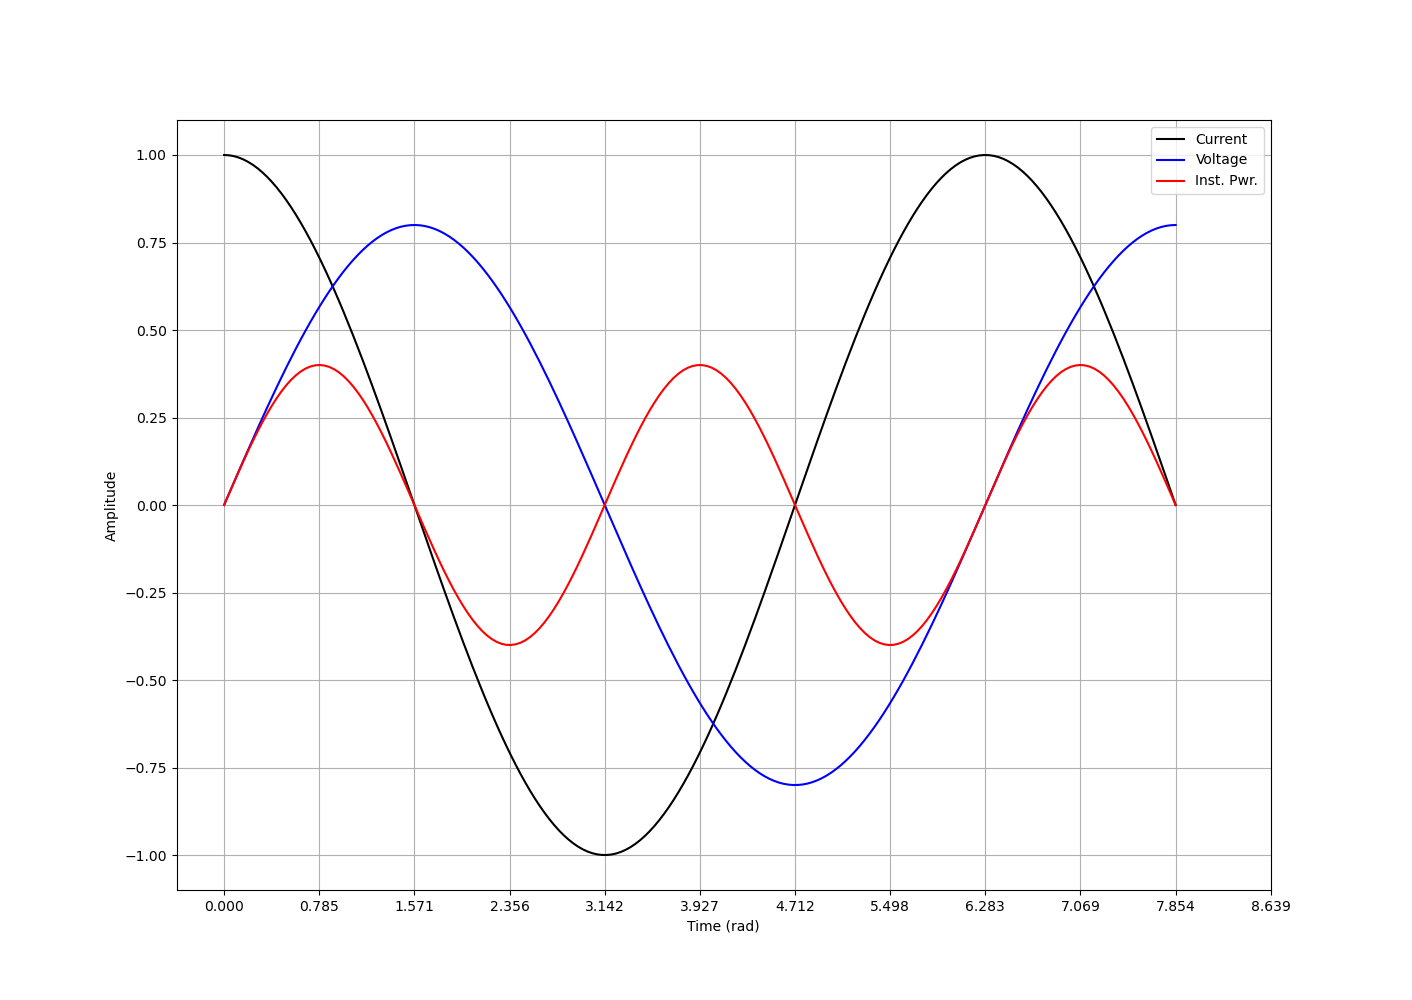
\includegraphics[width=0.5\textwidth]{figsChapt03/US73216.png}  %2-Oct-25

Observations:
\begin{enumerate}
    \item The frequency of power (red plot) is double the frequency of the voltage and current ($2\omega$).
    \item The power is   positive for the same amount of time as it is
    negative and has a smooth sinusoidal shape, so its average value
    (area under the wave divided by time), is zero.
    \item At a short time scale however power is alternating between
    positive and negative.  This means energy is alternately flowing
    into and out of the {\bf capacitor's electric field}.
\end{enumerate}

\subsection*{Resistor}

With a resistor of course voltage and current are related by
  $\vec V = \vec I R$ where $R$ is a real number.  Therefore the voltage and current sinusoids are perfectly in phase.
\[
Z = R \quad V_M = I_M R \quad \angle Z = \phi = 0
\]

\[
p(t) = \frac{I_M^2 R}{2} + \frac{I_M^2 R}{2} \cos(2\omega t + \phi)
\]
Observations:
\begin{enumerate}
    \item The frequency of power is double the freqency of the voltage and
    current ($2\omega$)
    \item The power is always positive at all times so it's average value
    (area under the wave divided by time), is non-zero and positive.
\end{enumerate}

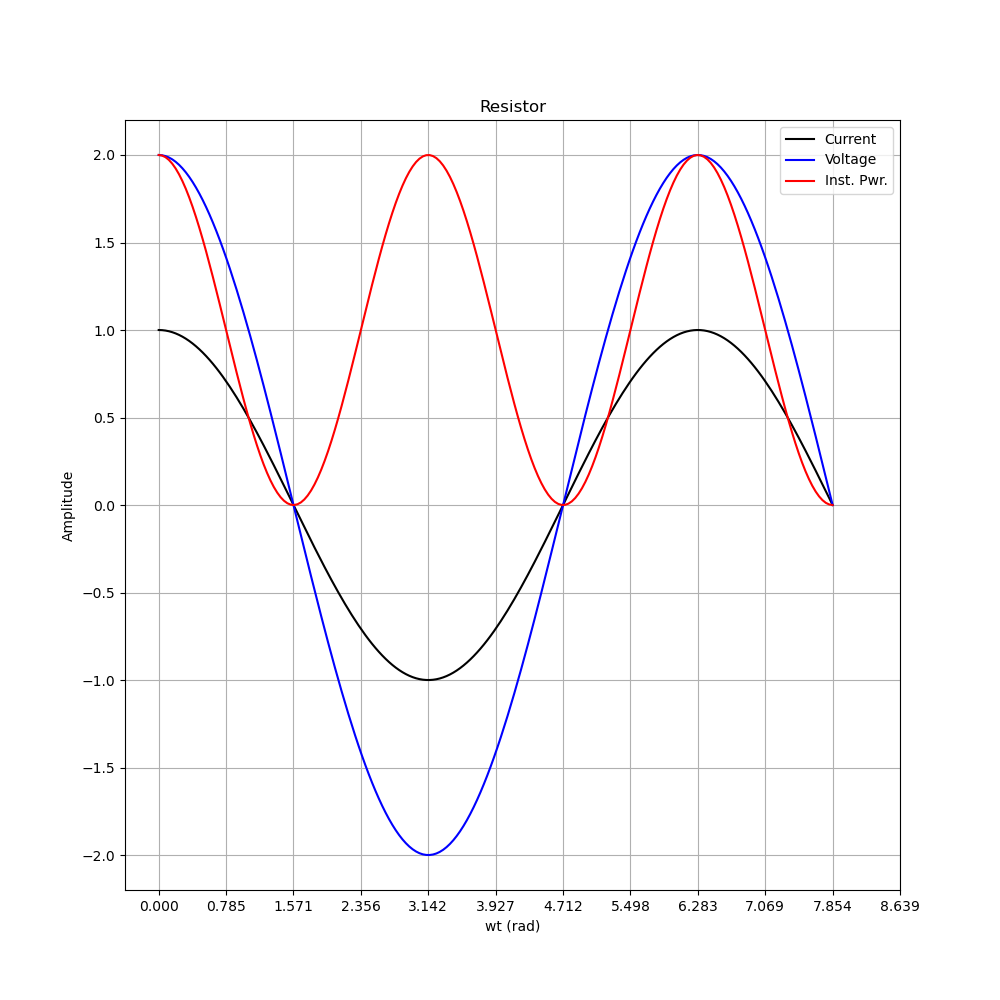
\includegraphics[width=0.5\textwidth]{figsChapt03/QI00215.png}

\subsection*{Inductor:}

Just as with the capacitor, the net power in an inductor is zero. (Note
different y-axis scale for this plot).
The phase shift is now $+\pi/2$ but the product of voltage and current
is still symmetrical about the $\omega t$ axis which averages to zero.

\[
Z = j\omega L \quad V_M = I_M \omega L \quad \angle z = \pi/2
\]

\[
p(t) = 0 + \frac{I_M^2}{2} \omega L \cos(2\omega t + 2\phi + \frac{\pi}{2})
\]

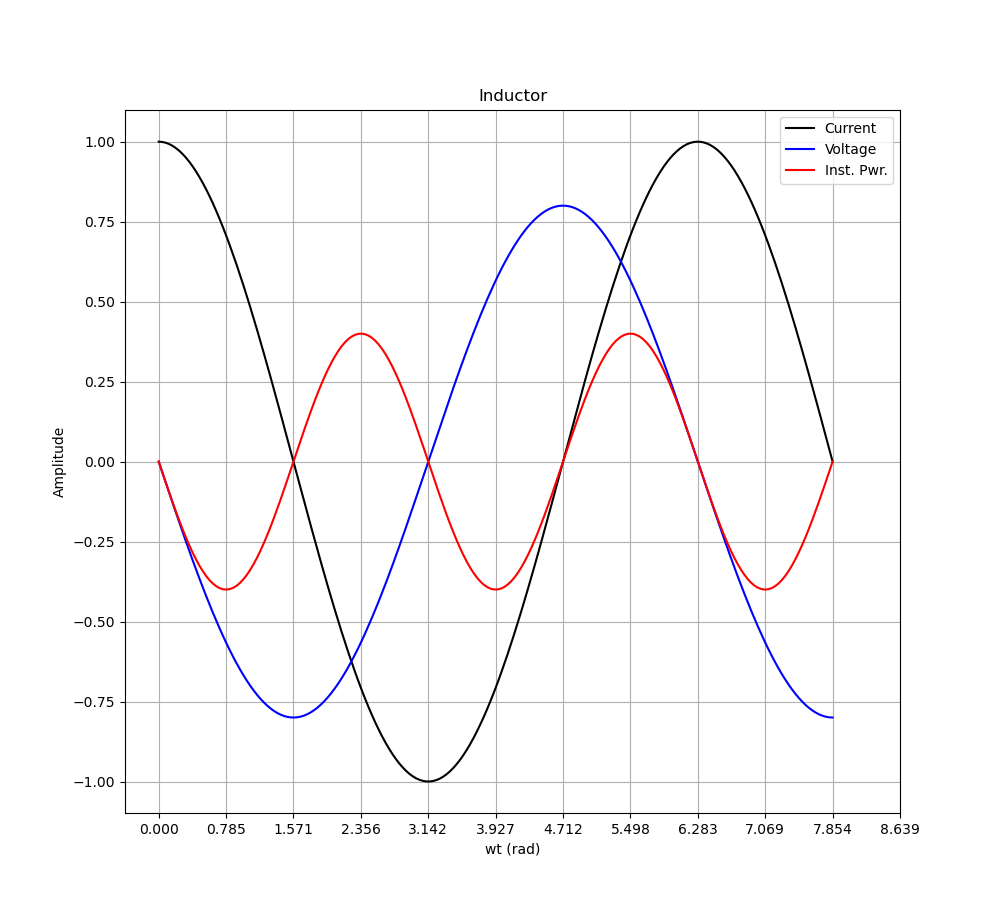
\includegraphics[width=0.5\textwidth]{figsChapt03/LN19448.png}


\begin{enumerate}
    \item The frequency of power (red plot) is double the frequency of the voltage and current ($2\omega$).
    \item The power is positive for the same amount of time as it is
    negative and has a smooth sinusoidal shape, so it's average value
    (area under the wave divided by time), is zero.
    \item At a short time scale however power is alternating between
    positive and negative.  This means energy is alternately flowing
    into and out of the {\bf inductor's magnetic field}.
\end{enumerate}




\subsection*{Example:}


Find the average power sourced by the voltage source in this circuit:


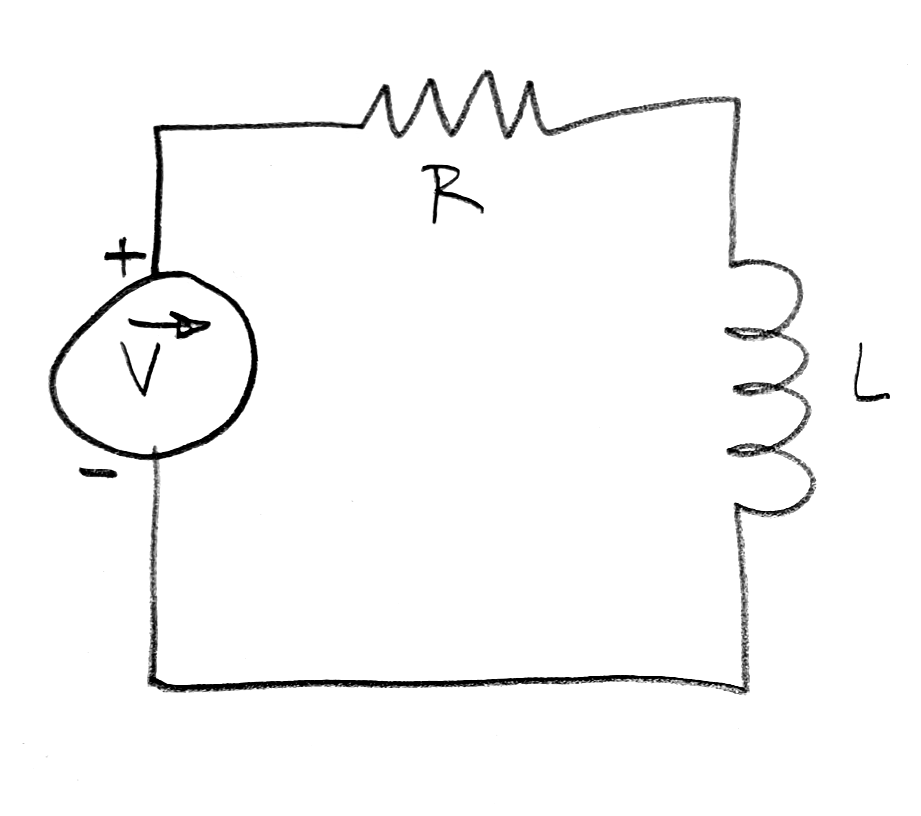
\includegraphics[width=0.4\textwidth]{figsChapt03/TU95372.png}


\[
\omega = 100 rad/s\;\; \vec{V} = 20 e^{j 0^\circ} = 20\; \mathrm{Volts}
\]

\[
R = 10 \Omega,\;\; L = 0.1 \text{H}
\]

\noindent Since $\vec V$ is a sinusoid (with an absolute magnitude of
$V_M=20$), we can apply

\[
P_{AV} = \frac{I_M V_M}{2} \cos(\phi)
\]
where $\phi$ is the phase difference between voltage  and current.

\[
\vec{I} = \frac{\vec{V}}{Z},  \quad \phi = \angle{Z}
\]

% applying Ohm's law and $\vec V_L = j\omega L$,
\[
Z = 10 + j10 = 10\sqrt{2}e^{j45^\circ}
\]
putting $Z$ and $I$ in mag/angle form:
\[
\vec{I} = \frac{\vec V}{Z} = \frac{20}{10\sqrt{2} e^{j45^\circ}} = I_M e^{j-45^\circ}
\]
\[\boxed{
    I_M=\frac{2}{\sqrt{2}}
  }
\]
\[
P_{AV} = \frac{I_M V_M}{2} \cos(\angle Z) = \frac {2}  {\sqrt{2}} \frac {20}  {2}\cos(-45^\circ)
\]
\[\boxed{
    P_{AV} = \frac {40}  {2\sqrt{2}}\cos(\angle Z)  =  \frac {20}  {\sqrt{2}}\times 0.707 = 10.9 \text{ Watts}
    }
\]


We call the factor $\cos(\angle Z)$ the {\bf power factor, PF}, a number
between 0 and 1 which determines how much average power we get from the
given voltage and current magnitudes.

Note that
\[
\mathrm{PF} = \cos\left(\tan^{-1}\left ( \frac {\mathrm{IM}\{Z\} }  {\mathrm{RE}\{Z\}}  \right ) \right) = \cos\left ( \angle{Z}\right )
\]
%
%
%
% \[
% \text{Note, } pf = \cos\left(\tan^{-1}\frac{\text{Im}(Z)}{\text{Re}(Z)}\right) = \cos(\angle Z)
% \]

\noindent Why?  Because

\[
\vec{V} = \vec{I} Z\;\; \text{ and }
\]
\[
\angle V - \angle I = \angle Z
\]

Let's apply this to
find $P_{AV}$ dissipated in the resistor $R$ of the above circuit

\[
\vec{I}_R = \vec{I}/\sqrt{2} = \frac{1}{\sqrt{2}} e^{j-45^\circ}
\]

\[
\vec{V}_R = \vec{I}_R R = \sqrt{10^2 +10^2}e^{j-45^\circ} =\frac{10}{\sqrt{2}} e^{j-45^\circ}
\]

therefore:
\[
 I_{mR} = \frac{1}{\sqrt{2}}, \quad V_{mR} = \frac{10}{\sqrt{2}}, \quad \phi = \angle Z = -45^\circ
\]

\[
P_{AVR} = \frac{10}{\sqrt{2}\sqrt{2} }   \cos(-45^\circ) = 3.535 \text{ Watts}
\]

\noindent Note

\[
P_{AVR} = P_{AV_{\text{TOTAL}}}
\]
What we computed for the resistor alone is also the total for
the whole circuit.

% Checking this, let's find $P_{AV}$ ``dissipated in'' L
%
% \[
% \vec{I}_L = \vec{I} = \frac{1}{\sqrt{2}} e^{j45^\circ}
% \]
%
% \[
% \vec{V}_L = j\omega L \vec{I} = e^{j\pi/2} \frac{10}{\sqrt{2}} e^{j45^\circ} = \frac{10}{\sqrt{2}} e^{j135^\circ}
% \]
%
% \[
% P_{AVL} = \frac{1}{\sqrt{2}} \cdot \frac{10}{\sqrt{2}} \cos(135^\circ - 45^\circ) = 0!
% \]
%
%
% This will always be true because
%
% \[
% \angle z_L = \pi/2 \Rightarrow pf_L = 0
% \]

\newpage

\subsection{Summarizing: Power in AC elements}

\begin{tabular}{|c|c|c|c|c|c|}
\hline
Element & $Z$ & $\angle z$ & $pf$ & $p(t)$ & $\phi $ \\
\hline
R & $R + j0$ & 0 & 1 & $\frac{I_M^2 R}{2} + \frac{I_M^2 R}{2} \cos(\omega t)$ & \\
 & & & & $P_{AV}$ & $  0$ \\
\hline
L & $0 + j\omega L$ & $+90^\circ$ & 0 & $\frac{I_M^2}{2} \omega L \cos(2\omega t + \pi/2)$ & \\
 & & & & & $\pi/2$ \\
\hline
C & $0 - \frac{j}{\omega C}$ & $-90^\circ$ & 0 & $\frac{I_M^2}{2\omega C} \cos(2\omega t -\pi/2)$ & \\
 & & & & & $-\pi/2$ \\
\hline
Z & $R + jX$ & $\tan^{-1}(\frac{X}{R})$ & $\cos(\angle z)$ & & $ \angle z $ \\
\hline
\end{tabular}

\noindent Capacitors and Inductors (ideal ones) cannot dissipate power. Can only accumulate it and give it back. Only R element can dissipate Power.



\subsection{Optional Topic: Superposition of Power}

Here we will think about the question, ``Can we compute
two powers from two different sources separately and add them together?''

We'll check a simple example:

%
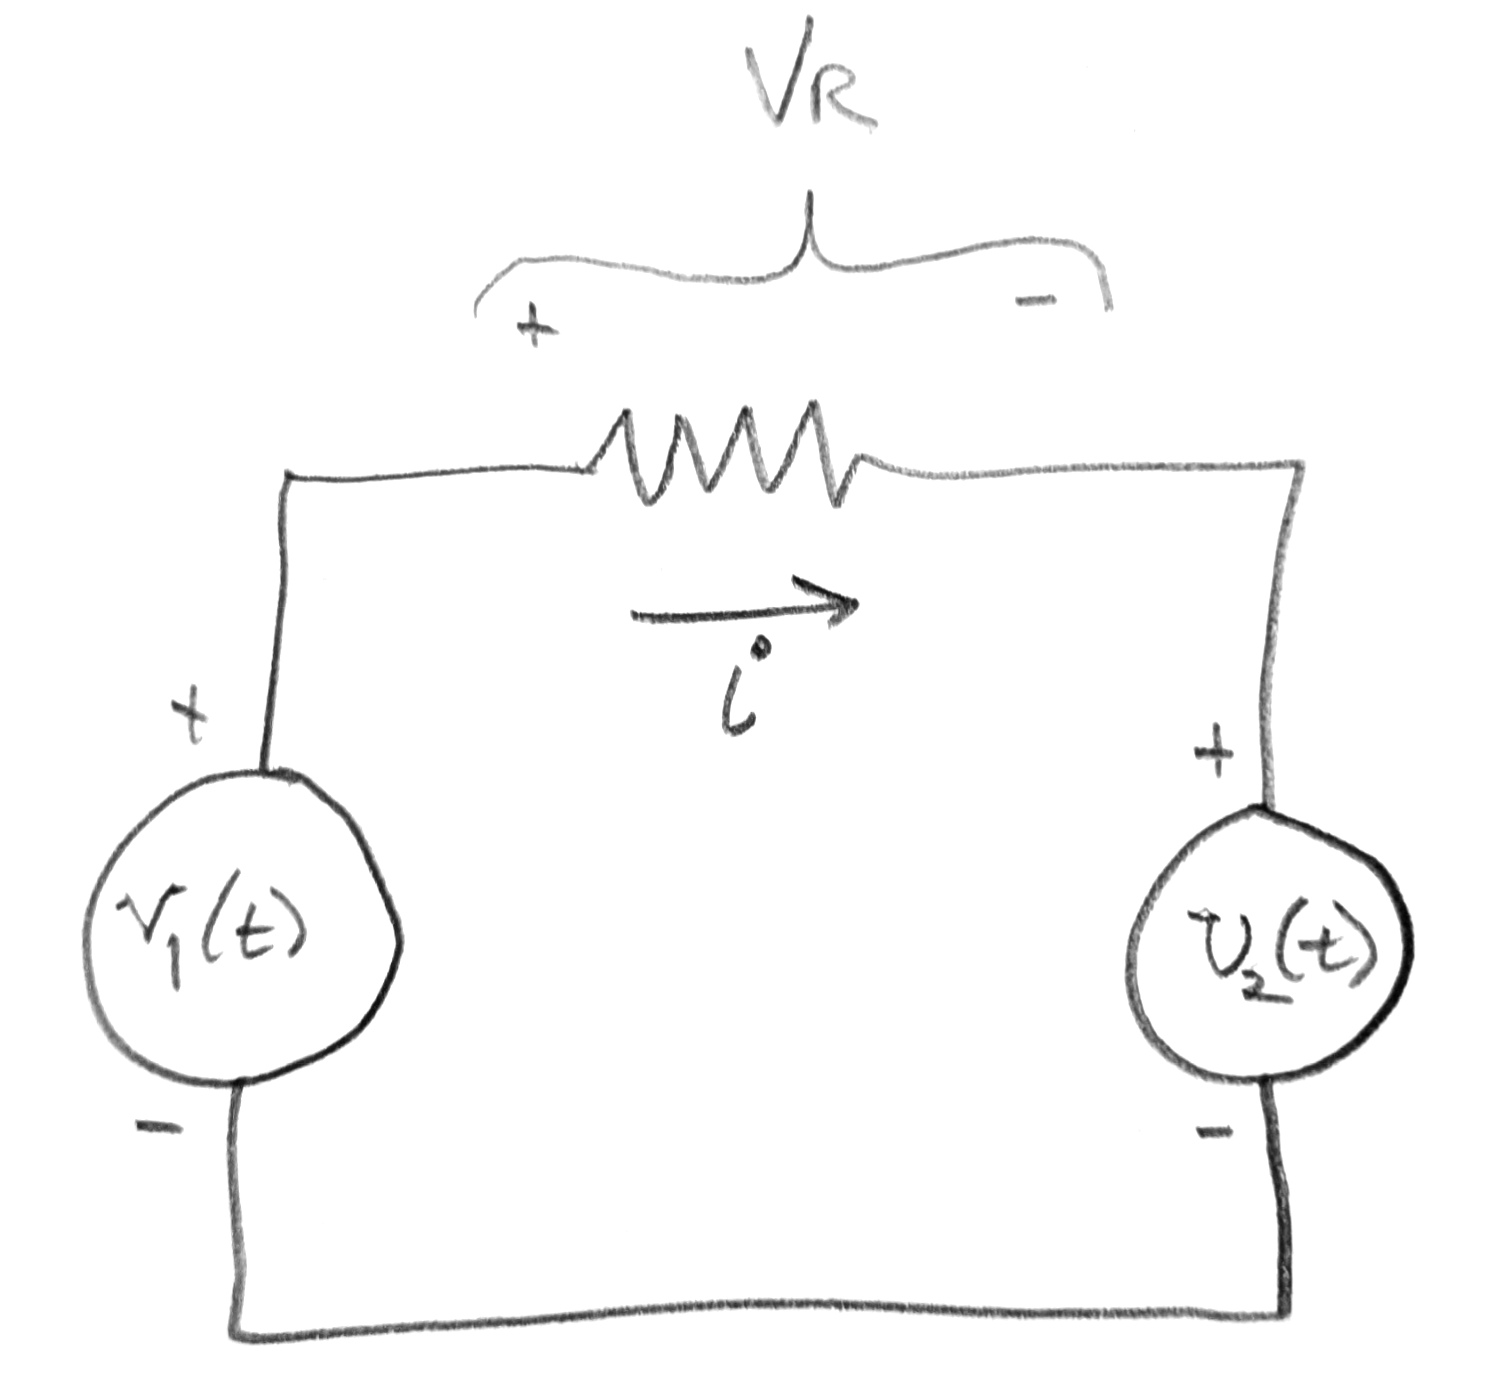
\includegraphics[width=0.4\textwidth]{figsChapt03/GP15083.png}



An approach based on superposition would say, let's set each
source to zero and compute the power delivered by the other source,
and then add them up, superimposing their solutions.
\[
i(t) = \frac{V_1(t)}{R} + \frac{V_2(t)}{R} = i_1(t) + i_2(t)
\]

using this sum to compute total power would give
\[
P(t) = i(t) V(t) \cdot R
= \left( i_1(t) + i_2(t) \right)^2 R
\]
\[
P(t) = \left( i_1^2(t) + i_2^2(t) \right) R + 2i_1(t) i_2(t) R
\]

But the last term means that we can't superpose power in this case at least.
But, suppose

\[
V_1(t) = V_1 \cos(\omega_1 t) \rightarrow i_1(t) = \frac{V_1 \cos(\omega_1 t)}{R}
\]

and
\[
V_2(t) = V_2 \cos(\omega_2 t) \rightarrow i_2(t) = \frac{V_2 \cos(\omega_2 t)}{R}
\]


where
\[
\omega_1 \neq \omega_2
\]

As we derived just above,
\[
P(t) = \frac{V_1^2 \cos^2(\omega_1 t)}{R} + \frac{V_2^2 \cos^2(\omega_2 t)}{R} + 2V_1 \cos(\omega_1 t) V_2 \cos(\omega_2 t) \frac{1}{R}
\]


We now need a new definition of average power because this $P(t)$ is not in general periodic.
For example, if $\frac{\omega_1}{\omega_2}$ is irrational, then the last term has no
exact period to integrate over.

We'll solve this for non-periodic signals  by

\[
P_{AV} = \lim_{\tau \rightarrow \infty} \frac{1}{\tau} \int_0^\tau p(t) \, d\tau
\]
(which of course also works for periodic
signals)

%continuing, we get
Taking this new average power of our superposition approach above, we get
\[
P_{AV} = \frac{1}{R} \lim_{\tau \rightarrow \infty} \frac{1}{\tau} \int_0^\tau \left[ V_1^2 \cos^2(\omega_1 t) + V_2^2 \cos^2(\omega_2 t) + 2V_1 \cos(\omega_1 t) V_2 \cos(\omega_2 t) \right] d\tau
\]
Let's call the three terms inside the integral (in brackets), $P_1, P_2, P_3$ in other words:
\[
P_{AV} =\frac{1}{R} \lim_{\tau \rightarrow \infty} \frac{1}{\tau} \int_0^\tau \left[
P_1 + P_2 + P_3 \right ] d\tau
\]

looking at $P_3$,  since $\omega_1 \neq \omega_2$,
\[
\frac{1}{R} \lim_{\tau \rightarrow \infty} \frac{1}{\tau} \int_0^\tau \left[ P_3 \right ] d\tau = 0
\]

\[
= P_{AV_1} + P_{AV_2} + \{ P_{12} = 0 \}
\]

The point is that if in the steady state sinusoidal case, if $\omega_1 \neq \omega_2$, we {\bf can} assume
superposition of power computation.

\subsection*{Significance of Superposition of power at different frequencies}

A circuit or system with input composed if many sinusoids can be analyzed w.r.t. avg power at each freq separately.  Examples of where we will use this include Audio, Communications,
and Control Systems.

 Conceptual Note: Voltages and currents of different frequencies are `orthogonal' in the sense that the power factor between them is zero.
 Thus no average power is dissipated in R by the product $v_1(t) v_2(t)$.

\noindent



\section{RMS Voltage and Current}
Recall: for sinusoids,
\[
P_{AV} = \frac{I_M V_M}{2} \cos(\phi)
\]

It is tempting to see this as a vector/dot product between voltage and current ($I_M V_M\angle \phi
$).

e.g.

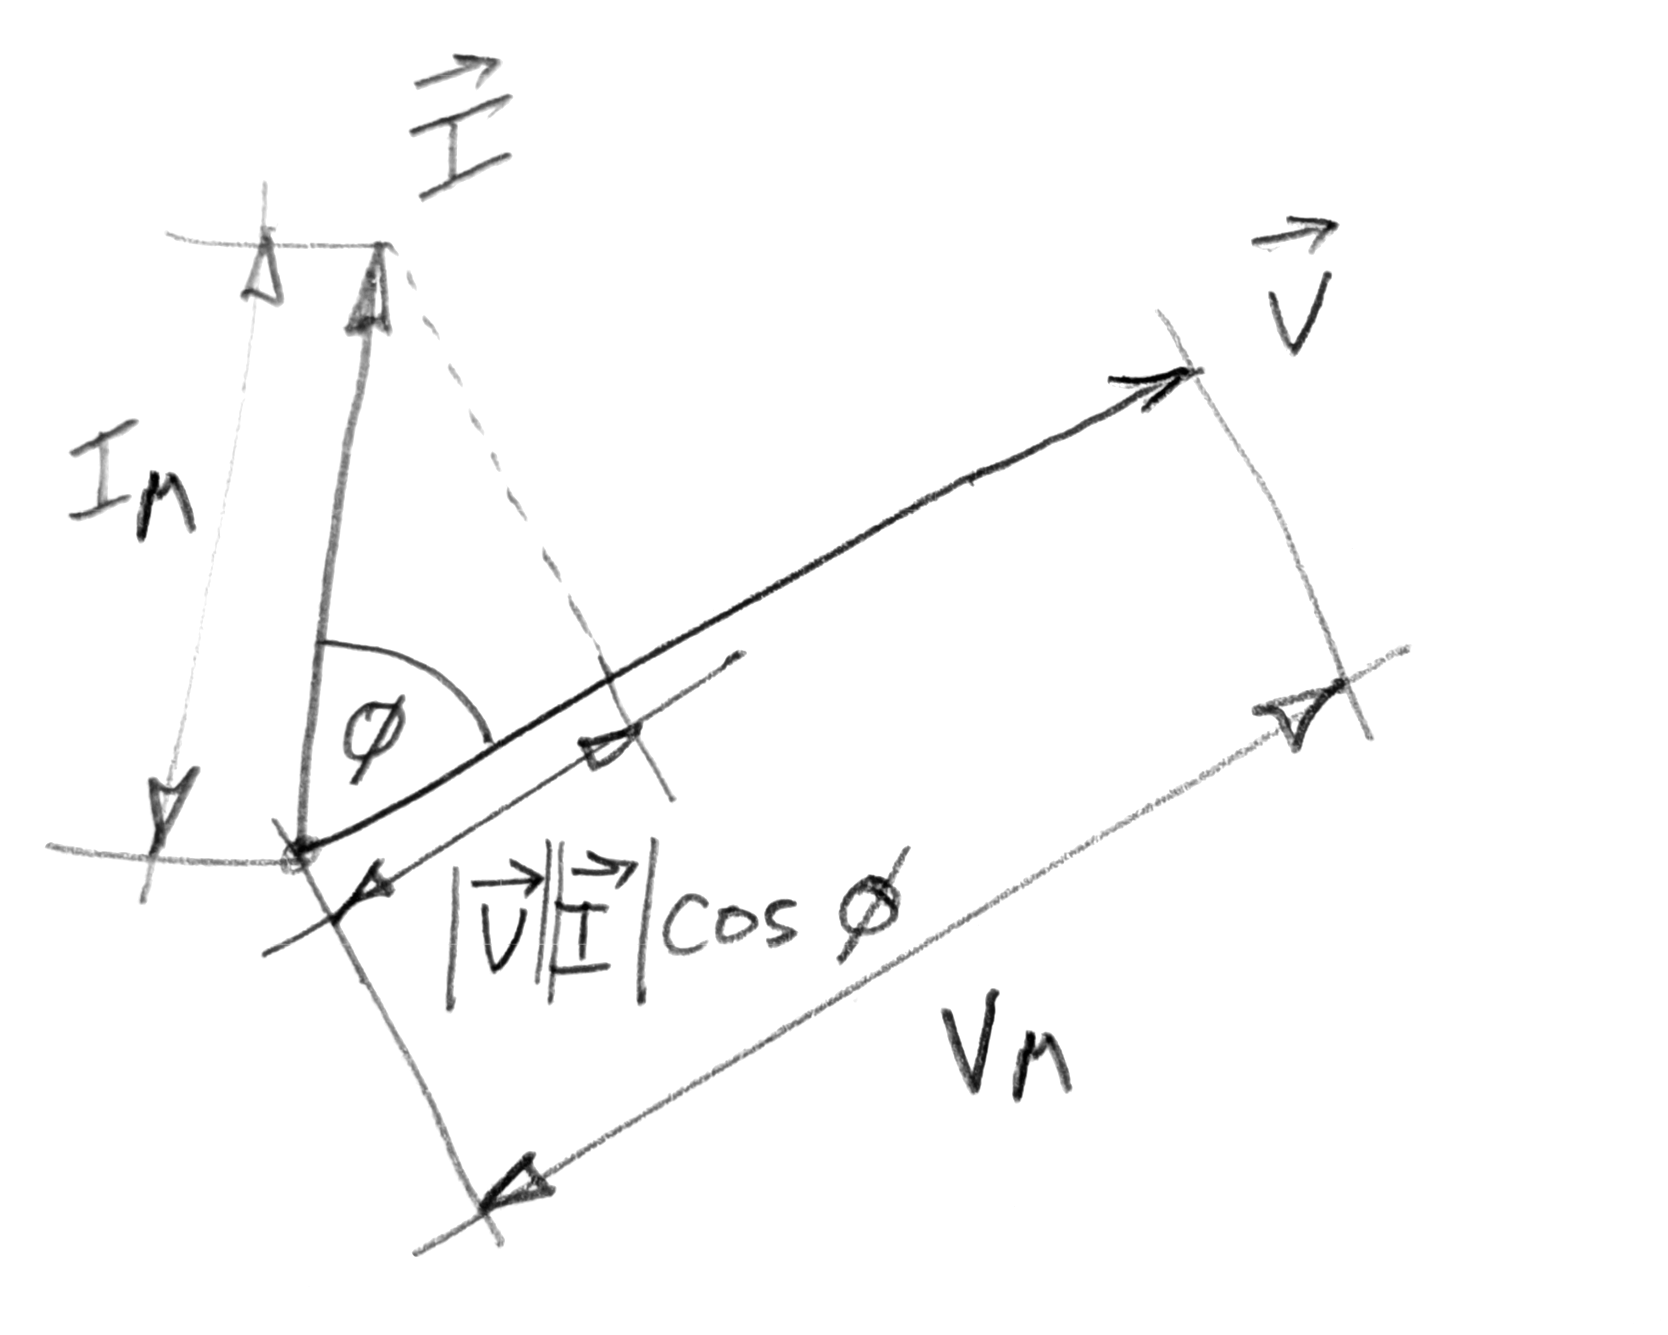
\includegraphics[width=0.3\textwidth]{figsChapt03/UH48274.png}

But, what about factor of $\frac{1}{2}$?    To allow this dot-product interpretation of
voltage and current phasors, we need a new concept, the {\bf Root-Mean-Square, RMS} voltage
and current.

For any function $x(t)$,

\paragraph{Define}

\[
\text{RMS}(x(t)) = \sqrt{\frac{1}{T} \int_0^T (x(t))^2 \, dt}
\]
Note that this equation takes
\begin{enumerate}
    \item {\bf R: } The square root of ...
    \item {\bf M: }the mean $\left ( \frac{1}{T} \int_0^T ... ,\;\; dt \right )$ of ...
    \item {\bf S: }The square of $x(t)$
\end{enumerate}

If
\[
v(t) = V_M \cos(\omega t + \alpha)
\]

then
\[
\text{RMS}(v(t)) = \sqrt{\frac{\omega}{2\pi} \int_0^{2\pi/\omega} V_M^2 \cos^2(\omega t + \alpha) \, dt}
\]


\[
=\sqrt{ \frac{1}{2} V_M^2 }
= \frac{1}{\sqrt{2}} V_M \equiv V_{MR}
\]

(where $V_M, V_{NR}$ are real numbers).
We now can  define new phasors,
\[
\vec V_R = \frac {1}  {\sqrt{2}}  V_M e^{j\phi_1}
\]
\[
\vec I_R = \frac {1}  {\sqrt{2}}  I_M e^{j\phi_2}
\]

Since for sinusoids we are really just multiplying the magnitude by $\frac {1}  {\sqrt{2}} = 0.707$ it's useful to remember
that  the magnitude of the RMS phasor is just
\[
V_{MR} = 0.707 V_M
\]

\[
\vec V_R = 0.707 \vec V
\]

$V_{MR}$ is also the RMS value of the sinusoid in the time domain
which looks like:

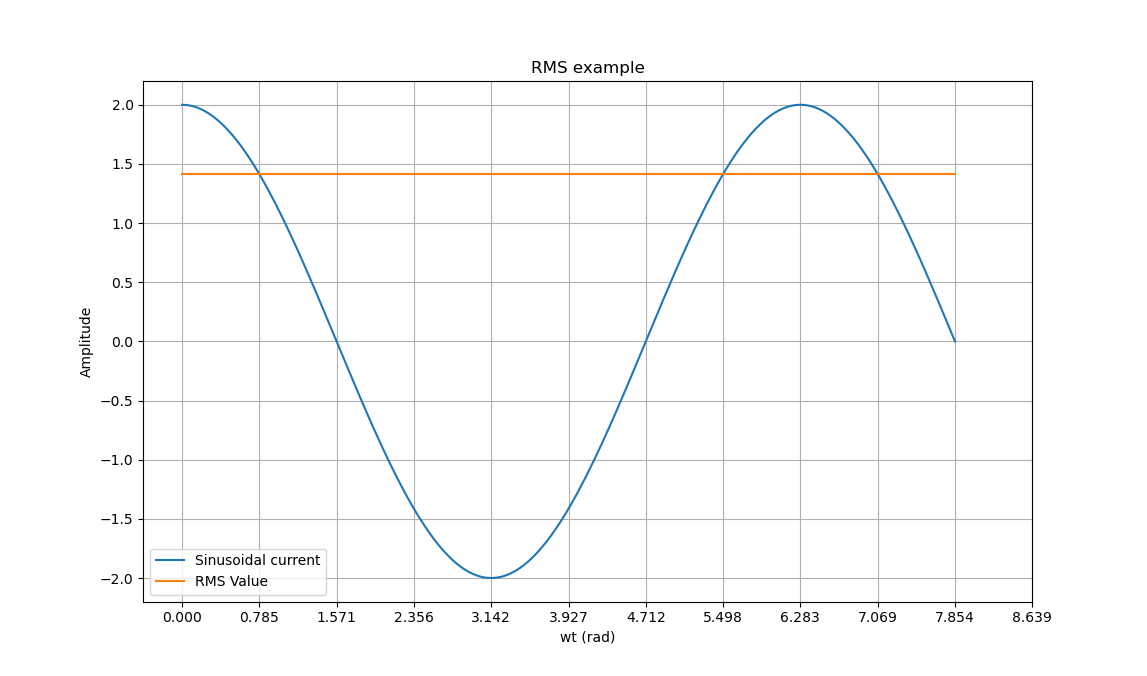
\includegraphics[width=80mm]{figsChapt03/FP56580.png}


Similarly
\[
\text{RMS}(i_R) = \frac{1}{\sqrt{2}} I_M \equiv I_R
\]

\noindent Also note,

\[
V_R I_R \cos(\alpha - \phi) = \frac{V_M I_M}{2} \cos(\alpha - \phi)
\]

\[
= P_{AV}
\]



\noindent Now $P_{AV}$ corresponds to vector dot product

%\includegraphics[width=0.4\textwidth]{figsChapt03/phasor_rms.png}

\[
\vec{V}_R, \angle(\alpha)
\]

\[
\vec{I}_R \angle(\phi)
\]


\paragraph{Example:}  Consider
120 $V_{RMS}$, also known as North American Household voltage
\vspace{0.25in}
\noindent Q: what is $V(t)$?
\vspace{0.25in}

\noindent A:
\[
\frac{V_M}{\sqrt{2}} = V_{RMS}
\]

\[
V_M = \frac{ 120 } {0.707} = 170
\]

\[
V(t) = 170 \cos(377t)
\]

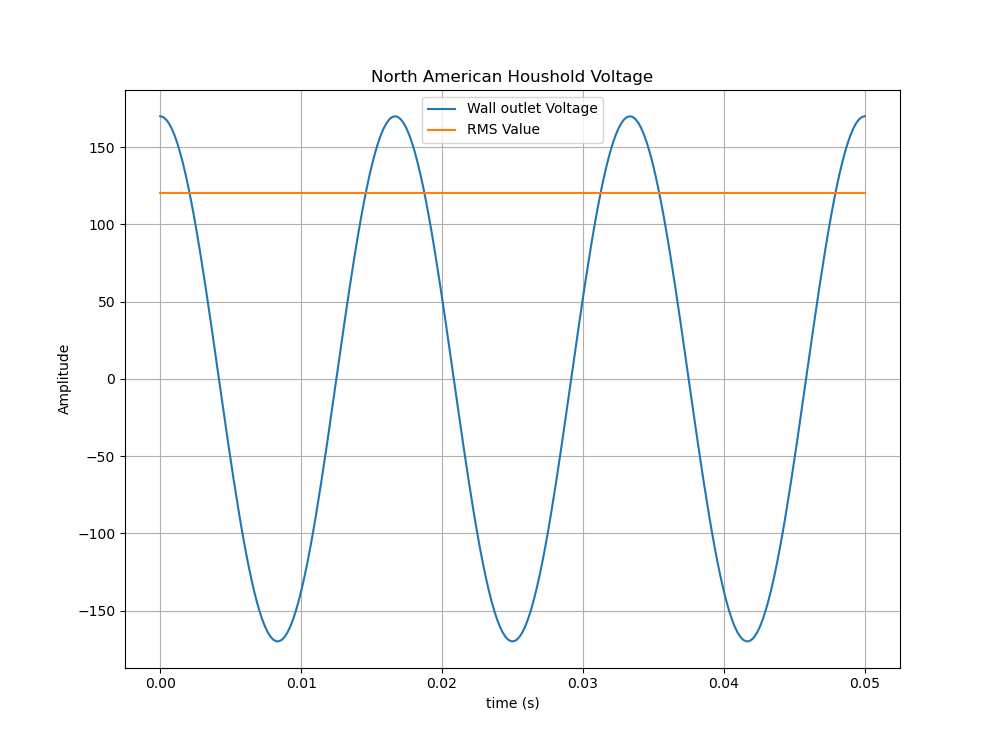
\includegraphics[width=0.5\textwidth]{figsChapt03/FM67804.png}



\subsection{RMS value of Non-Sinusoidal Pulse Train}
RMS value is not just for a sinuosoid.  It can be computed for any signal/waveform.
For example, let $V(t)$ be a train of rectangular pulses (between 0 and $A$ amplitude)
whose width can vary
independently of the period   as graphed below:


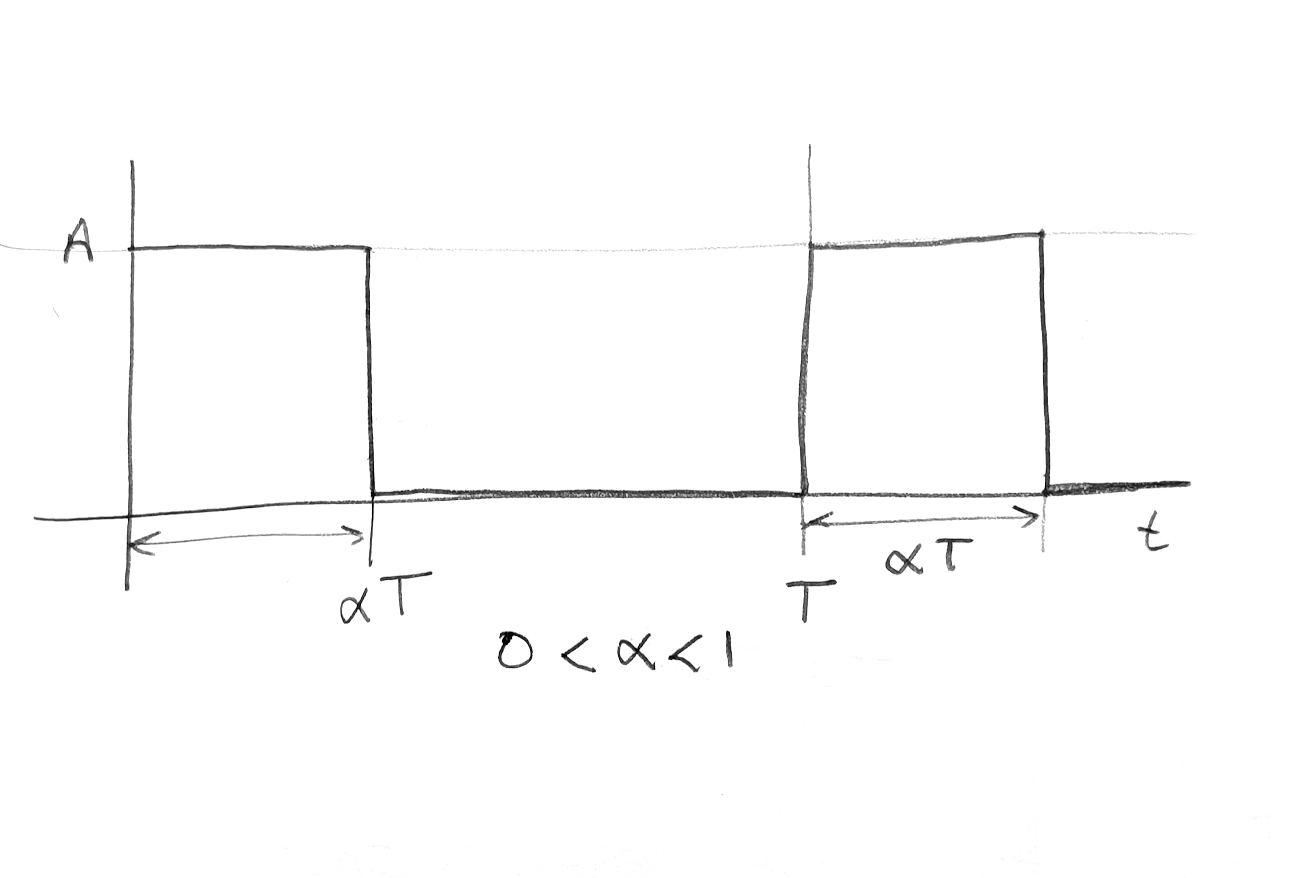
\includegraphics[width=0.5\textwidth]{figsChapt03/HT21139.png}


We call $\alpha $ the ``duty cycle'' \quad $0 \leq \alpha \leq 1$ which defines
how long the pulse lasts compared to the period, $T$.

\[
V_{RMS} = \sqrt{\frac{1}{T} \int_0^T V^2(t) \, dt}
\]

\[
= \sqrt{\frac{1}{T} \left[ \int_0^{\alpha T} A^2 \, dt +  \int_{\alpha T}^T 0^2 \, dt \right]}
= \sqrt{\frac{A^2}{T} [\int_0^{\alpha T} 1 \, dt] }
\]
\[
=\sqrt{\frac{A^2}{T} [ \alpha T] }= A\sqrt{\alpha}
\]

Note when
\[ \alpha = \frac{1}{2} \quad V_{RMS} = \frac{A}{\sqrt{2}}
\]
which is the same as a sinusoid for the amplitude.  But it's mean is non-zero
compared to a zero-mean for a sinusoid.








\subsection{Additional Forms:  Power for Sinusoids}
With the RMS value, we now have

\[
P_{AV} = V_R I_R \cos(\angle z)
\]

\noindent Note also

if $Z = R + jX \rightarrow$

%\includegraphics[width=0.3\textwidth]{figsChapt03/impedance_diagram.png}

\[
\cos(\angle z) = \frac{R}{|Z|}
\]

\[
P_{AV} = \frac{V_R I_R}{\sqrt{2}} \frac{I_R}{\sqrt{2}} \cdot \frac{\text{Re}(Z^*)}{|Z|}
\]

\[
= \frac{I_R^2}{2} \text{Re}\{Z^*\}
\]

\[
P_{AV} = \frac{I_M^2}{2} \text{Re}\{Z^*\}
\]

So it is important to realize that  RMS Voltages and currents can
be viewed as analogous to
equivalent DC voltage/current such that
\[
P_{AV} = \vec I_R\times \vec V_R
\]


 We now have:

\[
P_{AV} = V_R I_R \cos(\angle z)
\]

  Note also that if

\[
Z = R + jX
\]

Like with any complex number,
\[
\cos(\angle Z) = \frac{R}{|Z|}
\]

Applying this to our average power result:
\[
P_{AV} = \frac{V_R I_R}{\sqrt{2}} \frac{I_M}{\sqrt{2}}  \frac{\mathrm{Re}\{Z\} }{|Z|}
\]
but
\[
\vec{I}_M = \frac{V_M}{Z}
\]

\[
= \frac{I_M^2}{2} \mathrm{Re}\left\{{Z}\right\}
\]



\subsection{RMS Phasors}   Using the RMS concept we can modify phasors to use
the RMS magnitude instead of absolute magnitude.

Take a voltage and current defined as

$i(t) = I_M \cos(\omega t + \phi)$

$v(t) = V_M \cos(\omega t + \phi + \angle z)$

Their phasors are
\[
\vec{I} = I_M e^{j\phi} \quad \vec{V} = V_M e^{j(\phi + \angle z)}
\]

\noindent Define ``RMS Phasor''

\[
\vec{I}_R = \frac{1}{\sqrt{2}} \vec{I} = \frac{I_M}{\sqrt{2}} e^{j\phi}, \quad \vec{V}_R = \frac{1}{\sqrt{2}} \vec{V} = \frac{V_M}{\sqrt{2}} e^{j(\phi + \angle z)}
\]

Let's multiply the RMS voltage phasor times the complex conjugate of the current
phasor ($\vec I_R^*$):

\[
\vec{V}_R \vec{I}_R^* = \frac{V_M I_M}{\sqrt{2}\sqrt{2}} e^{j(\phi + \angle z)} e^{-j\phi}
\]
(note how the CC changed the sign of $e^{-j\phi}$ exponent)

\[
= \frac{V_M I_M}{2} e^{j\angle z}
\]

Taking the real part of this complex number:
\[
\quad \text{Re}\{\vec{V}_R \vec{I}_R^*\} = \frac{V_M I_M}{2} \cos \angle z = P_{AV}
\]
Bottom line is we get the average power directly by multiplying RMS voltage phasor
times the complex conjugate of the current phasor.






\section{ ``Complex Power''}






We define a complex quantity
\[
S = P + jQ \equiv \vec{V}_R \vec{I}_R^*
\]
as the {\bf complex power} in a circuit.

For the RMS phasors:
\[
\vec V_R = V_Re^{j0},\;\vec I_R=I_Re^{j\phi}
\]
(we can assume the voltage phase is zero without loss of generality. Otherwise
$\phi = \theta_V - \theta_I$, and remember that $\phi = \angle{Z}$.)
The real and imaginary parts of $S$ are:
\[
P = \text{Re}\{\vec{V}_R \vec{I}_R^*\} = P_{AV} = V_R I_R \cos \angle Z
\]

\[
Q = \text{Im}\{\vec{V}_R \vec{I}_R^*\} = V_R I_R \sin \angle Z
\]

$P$ is the {\bf Real Power}

$Q$ is the {\bf Reactive Power}

Complex power can be plotted on the complex plane.  The Real Power, $P$, is
the real-axis component, and the Reactive Power, $jQ$ is the imaginary component
of Complex Power.

\vspace{0.25in}
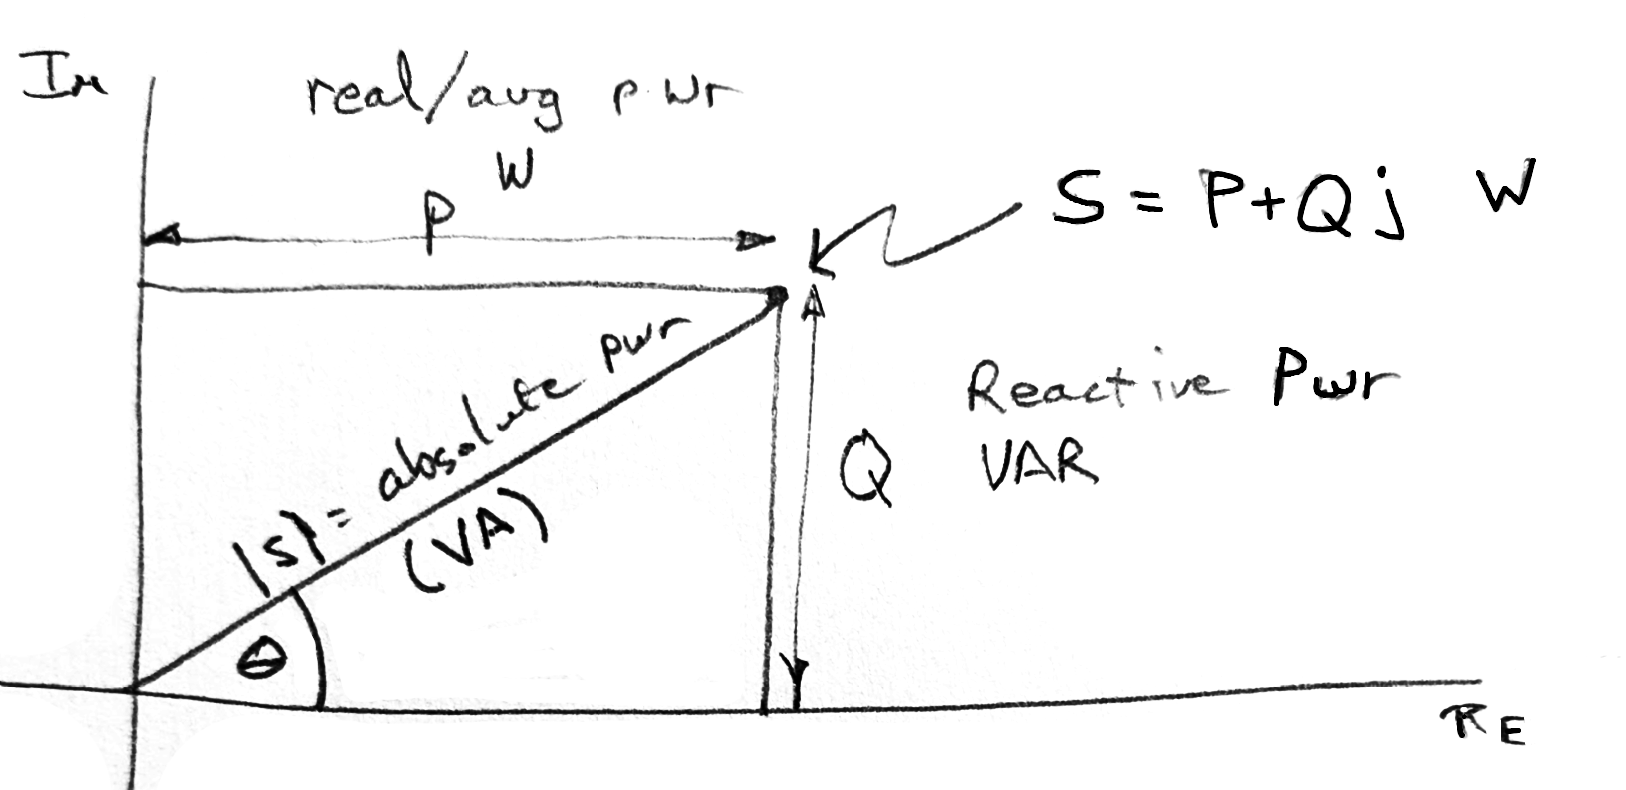
\includegraphics[width=0.65\textwidth]{figsChapt03/A69D31.png}

Where $\theta = \angle{Z}$.

\subsection{Types of Power }
Summarizing the types of power so far!

\begin{center}
\begin{tabular}{|c|c|c|}
\hline
Type & Definition & Unit \\
\hline
Complex  & $S=P+jQ$   &  VA "Volt-Ampere"  \\
Real & $P_{AV}$, $\text{Re}\{S\}$, & Watts \\
 & $\frac{I_M^2}{2} \text{Re}\{Z\}$ etc. & \\
\hline
Reactive & $\text{Im}\{S\}$ & VAR ``Volt Ampere Reactive'' \\
 & $V_R I_R \sin \angle z$ etc. & \\
\hline
Apparent & $V_R I_R$ & VA ``Volt Ampere'' \\
\hline
\end{tabular}
\end{center}

Some facts obvious from the complex power diagram above:
\begin{enumerate}
\item Apparent Power $\geq$ Real Power
\item Apparent Power $\geq$ Reactive Power
\item Apparent Power $\leq$ Real Power + Reactive Power
\end{enumerate}








\subsection{Two Ways to get Complex Power in an Impedance}

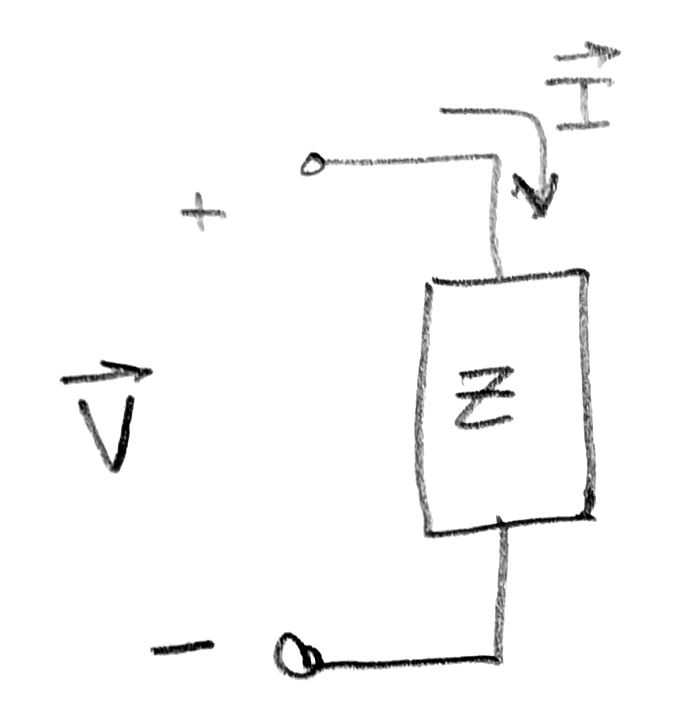
\includegraphics[width=0.3\textwidth]{figsChapt03/MB87549.png}

1)
\[
 \quad S = \vec{V}_R \vec{I}_R^*,
\]
and,
\[
\vec{I}_R^* = \frac{\vec{V}_R^*}{Z^*}
\]

\begin{ExampleSmall}
Where we have used the following trick:

\noindent
Show that
\[
\left (\frac {a}  {b}\right )^*  =  \frac {a*}  {b*}
\]
where $a = ar+ja_i, b = br+jb_i$
\[
\left (\frac {a}  {b}\right )*  =  \left (\frac {ar+j a_i}  {br+jb_i} \right )^* =
\left (\frac {|a|}  {|b|} (\angle a - \angle b) \right )^*
\]
\[
= \left (\frac {|a|}  {|b|} (\angle b - \angle a) \right )
\]
\[
=\frac {|a|\angle b}  {|b|\angle a}
=\frac {|a|\angle -a}  {|b|\angle -b}
\]
showing that
\[
\left (\frac {a}  {b}\right )^*  =  \frac {a*}  {b*}
\]
\end{ExampleSmall}
\vspace{0.25in}

So
\[
S = \frac{\vec{V}_R \vec{V}_R^*}{Z^*} = \frac{|\vec{V}_R|^2}{Z^*}
\]
\[\boxed{
= \frac{V_M^2}{\vec{2}}\frac{1}{Z^*}
}
\]

2)
\[
\vec{V}_R = \vec{I}_R Z
\]

\[
S = \vec I_R \vec I_R^* Z
\]

\[
= |\vec{I}_R|^2 {Z} = I_R^2 {Z}
\]
\[
\boxed {
     S=  \frac{I_M^2}{2} {Z}
     }
\]

Notes:
\begin{itemize}
\item In both cases, $\angle S = \angle Z$

\item RMS current and voltage phasors can be used like DC voltage and current where

$R$, Resistance, $ \rightarrow Z$

$A^2$, Currrent squared, $ \rightarrow A A^* = |A|^2$
\end{itemize}

Summarizing:

\begin{center}
\begin{tabular}{c|c}
DC & RMS sinusoids \\
\hline
$P = I^2 R$ & $S = |\vec{I}_R|^2 Z$ \\
$P = \frac{V^2}{R}$ & $S = \frac{|\vec{V}_R|^2}{Z^*}$ \\
\end{tabular}
\end{center}





\subsection{Conservation of Complex Power}

\noindent Consider

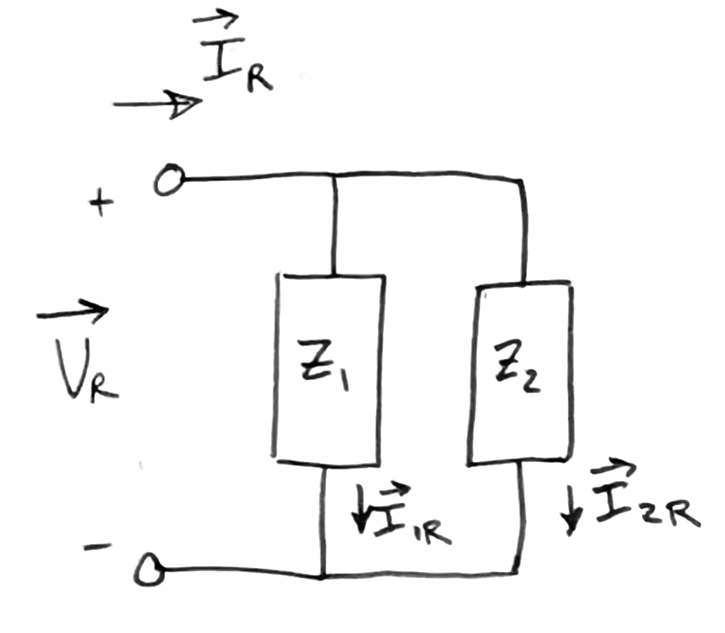
\includegraphics[width=50mm]{figsChapt03/QM27615.png}

by KCL, (+ = leaving the node).   By $\vec V_R$ and $\vec I_R$ we mean
the RMS phasors for voltage and current.

\[
-\vec{I}_R + \vec{I}_{1} + \vec{I}_{2} = 0
\]


\[
\vec{I}_R = \vec{I}_{1} + \vec{I}_{2}
\]

\[
S = \vec{V} \vec{I}_R^* = \vec{V}_R (\vec{I}_{1}^* + \vec{I}_{2}^*)
\]

\[
= S_1 + S_2
\]

In other words, the power entering the circuit is the sum of the power in
$Z_1$ plus the power in $Z_2$.



\noindent Also consider the series circuit:

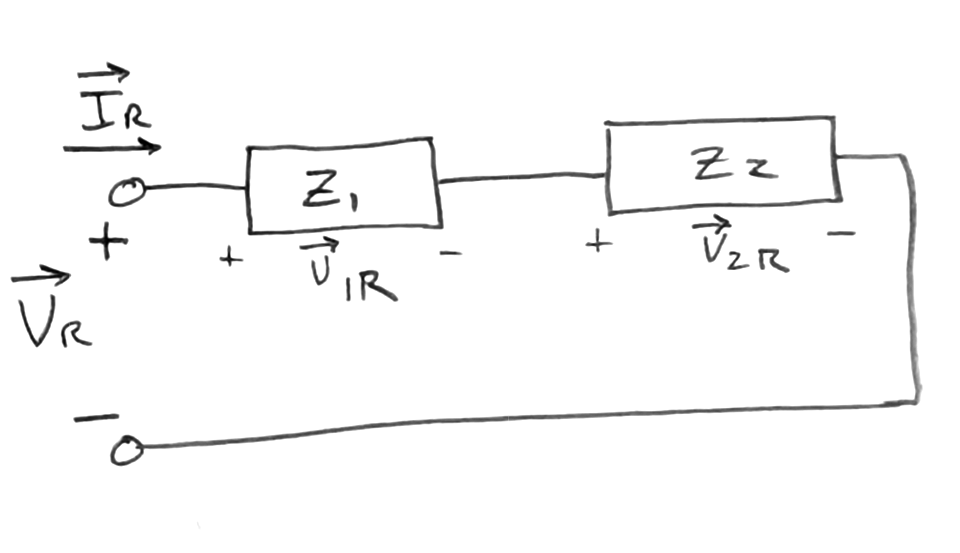
\includegraphics[width=80mm]{figsChapt03/RQ15238.png}

(where all quantities shown are RMS values.)
Using KVL:

\[
-\vec{V}_R + \vec{V}_{1R} + \vec{V}_{2R} = 0
\]

\[
 \vec{V}_R = V_{1R} + V_{2R}
\]

\[
S = \vec{V}_R \vec{I}_R^* = (\vec{V}_{1R} + \vec{V}_{2R}) \vec{I}_R^*
\]

\[
= S_1 + S_2
\]

Again, the complex power in whole circuit can be obtained by
adding complex power in each Z.  Which seems to agree with physical
intuition.




\subsection{Application: Power Factor Correction}

A power plant supplies electric power to a load over a long transmission line.
The transmission line has resistance, $R$.

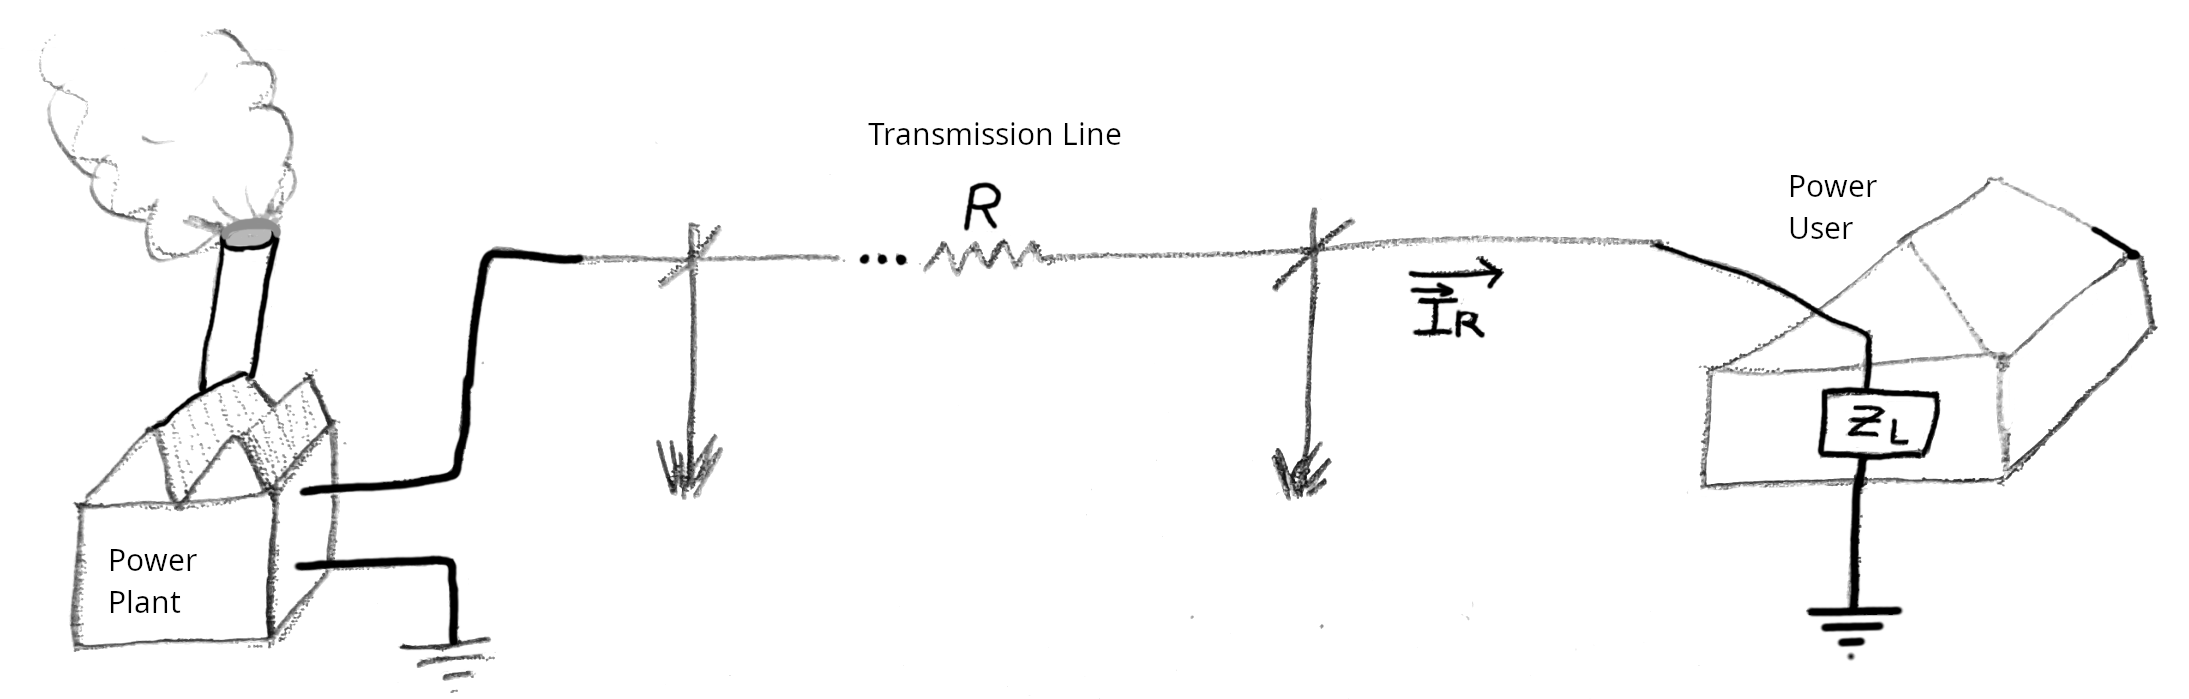
\includegraphics[width=\textwidth]{figsChapt03/BN97423.png}


The power company collects revenue based on the average power delivered
to the customer (as that is what is measured by the electric meter, see below).


\[
P_{AV_{\text{user}}} = \text{Re}\{S_{\text{user}}\} \equiv  \$
\]

But the power plant sees an additional load which is dissipated in the
resistance of the transmission line.


\[
P_{\text{plant}} = \text{Re}\{S_{\text{user}}\} + |\vec{I}_R|^2 R
\]


The last term above is loss in the transmission line and the utility needs
 to minimize it because the user's meter does not see it.

Our user load is
\[
Z_L = R + jX
\]

Typically loads are more inductive, i.e. $X>0$.  Also we know that
\[
X>0,\;\; \theta = \angle Z_L > 0, \;\; \text{pf} < 1
\]

The user is paying for
\[
P_{AV_{\text{user}}} = \text{Re}\left\{ |\vec{I}_R|^2 Z_L \right\}
\]

\[
= \text{Re}\left\{ |\vec{I}_R| |Z_L| (\cos \angle z_L + j \sin \angle z_L) \right\}
\]

\[
= |\vec{I}_R| |Z_L| (\cos \theta)
\]

\noindent Assume constant power use,$P_{AV_{\text{user}}} = P$.

The wasted energy is the heating of the transmission line which is  $R|\vec{I}_R|^2$,
so how does $\vec{I}_R$ depend on the power factor of $Z_L$?
From the previous result:

\[
|\vec{I}_R|^2 = \frac{P}{|Z_L| \cos \angle z_L}
\]

Summing up, for fixed user power, $P$ and $Z_L$, the power lost in
the transmission line, $|\vec{I}_R|^2 R$, is minimized (but not eliminated) when

\[
\cos \angle z_L = 1
\]

So if the user can ``correct'' their power factor towards 1.0,
the utility saves money.
For this reason, utilities often can charge
an extra fee to users whose power factors fall below a  threshold.

We move the power factor towards 1 by moving the
impedance angle to 0.
Looking at this graphically, suppose our power factor is too low because
the user's impedance ($Z_L$) has too much positive (inductive) reactance:

\vspace{0.15in}
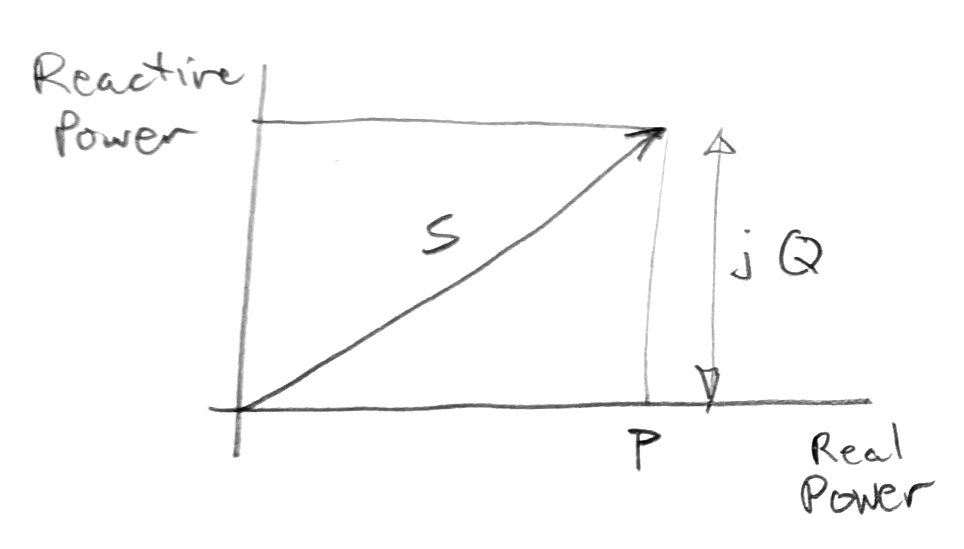
\includegraphics[width=70mm]{figsChapt03/KM41864.png}

\[
Z_L = R + j\omega L
\]
\[
S = P + jQ_L
\]



Let's add a capacitor, $ C$  in parallel.

% ID44718
\vspace{0.1in}
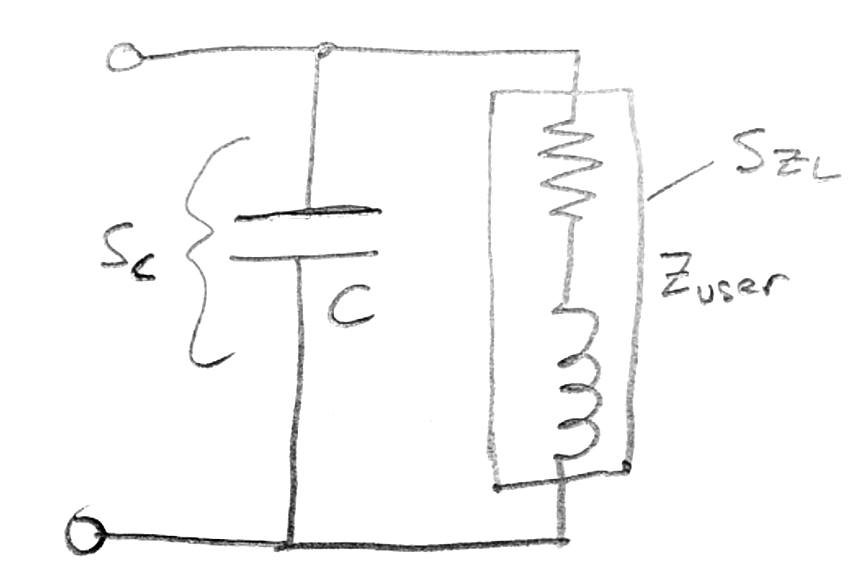
\includegraphics[width=60mm]{figsChapt03/ID44718.png}
\vspace{0.1in}

We've seen that the total complex
power is the sum of that in each of the two parallel branches:

\[
S = S_C + S_{Z_L}
\]

The power in the capacitor is a pure reactive power:
\[
S_C = 0.0 + j Q_C
\]
we don't know it's magnitude yet, only that it is pointing in the $-j$ direction
in the complex plane.   Lets suppose the inductive and capacitive reactances add
as shown below

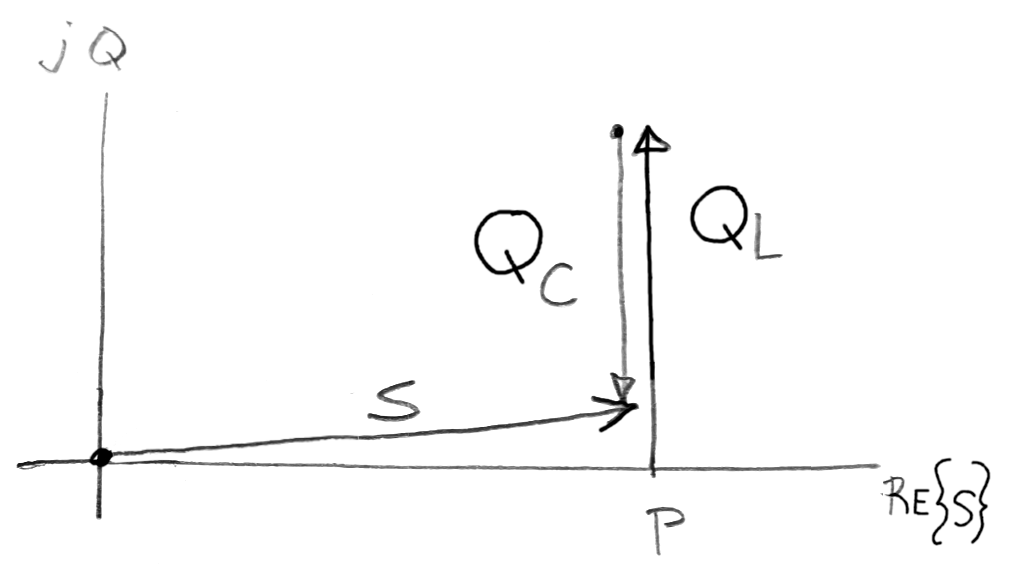
\includegraphics[width=70mm]{figsChapt03/MF77903.png}

(i.e $|Q_C| < |Q_L|$)

Now we have a much smaller {\bf net} inductive reactance.   We have ``corrected''
the power factor of the load to a more acceptable level.

It can be shown that  if we want a desired power factor of $pf_d$ and that our phase
angle is therefore $\theta_{pfd} = \cos^{-1}(pf_d)$ that

\[
C = \frac{Q_L - P \tan \theta_{pfd}}{\sqrt{|\vec{VL}_R|^2} \omega}
\]
%
% were $VL_R$ is the RMS load voltage.
%
% % \hspace{4cm} look at pg 485
% %
% %
% % \noindent Problem 12.2.2
%
% %\includegraphics[width=0.5\textwidth]{figsChapt03/problem_circuit.png}
%
% \[
% < z_{TH}
% \]
%
% \[
% P_{AV_{\text{Source}}} = P_{AV_{AC}} + P_{AV_{DC}}
% \]
%
% by superposition of power
%
% at diff freq
%
% \[
% = \left\{ \text{Re}\{\vec{V}_{2R} \vec{I}_{2R}^*\} \right\} + \frac{2\pi}{T} \int_0^{2\pi/T} \left\{ 50 \cdot 0.1 \cos(1000t) \right\} dt
% \]
%
%
% \[
% = -\text{Re}\left\{ \vec{I}_{2R} Z_{TH} \vec{I}_{2R}^* \right\} + \frac{10}{1000} \int_0^{1000/2\pi} \left( \cos(1000)dt \right)
% \]
%
% \[
% = -\text{Re}\left\{ |\vec{I}_{2R}|^2 Z_{TH} \right\}
% \]
%
% \hspace{5cm} 0
%
% \[
% Z_{TH} = 500 \parallel -j1000 = 400 - 200j
% \]
%
% \[
% P_{AV_{\text{Source}}} = -\text{Re}\left\{ 0.005(400 + 200j) \right\}
% \]
%
% \[
% = -2 \text{ Watts }
% \]

%
% \noindent (Pages 8-10 appear to be magazine/newspaper clippings about power systems and the "Power plus" UW invention for boost delivery efficiency, not handwritten notes. I'll skip those.)


\subsection{Power Meters}

\begin{center}
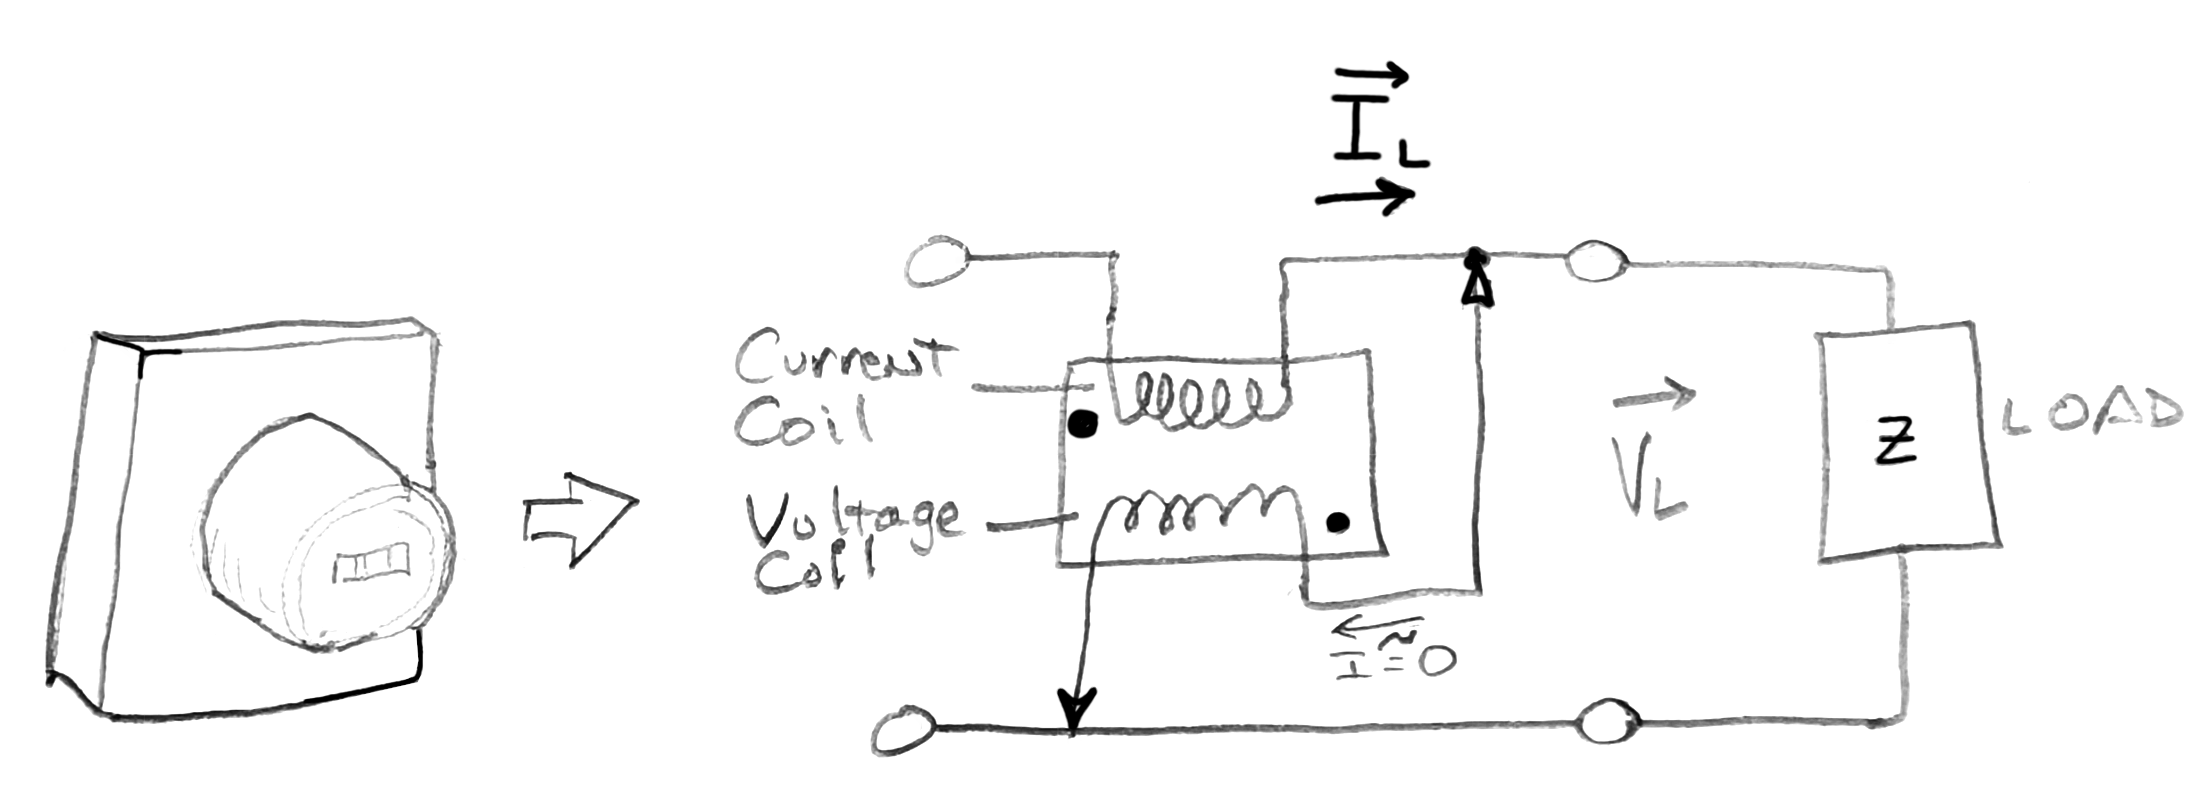
\includegraphics[width=120mm]{figsChapt03/TS44996.png}
\end{center}


The traditional electric meter has two coils, the ``voltage coil'' in parallel
with the load, to sense voltage, and the ``current coil''
in series to sense current.   Together they drive a rotating disk at a rate proportional
to voltage times current.
The black dot indicates the correct polarity for a
positive power reading when power is absorbed by $Z_L$.


To the extent the meter is ideal, the impedances of the two coils are:
\[
Z_{cc} = 0
\]
\[
Z_{vc} = \infty
\]
so that they do not distort the measurement or consume much energy themselves.



The two coils drive a disk who's angular velocity is
proportional to real power.   Gears integrate the  velocity to the indicator dial
positions\footnote{Today a digital circuit might count revolutions and display
a number on an LCD instead.}.

When the load is wired according to the diagram with the correct polarity,

\[
V_{disk} \propto V_{LR} I_{LR} \cos \angle Z_L
\]



\begin{Example}


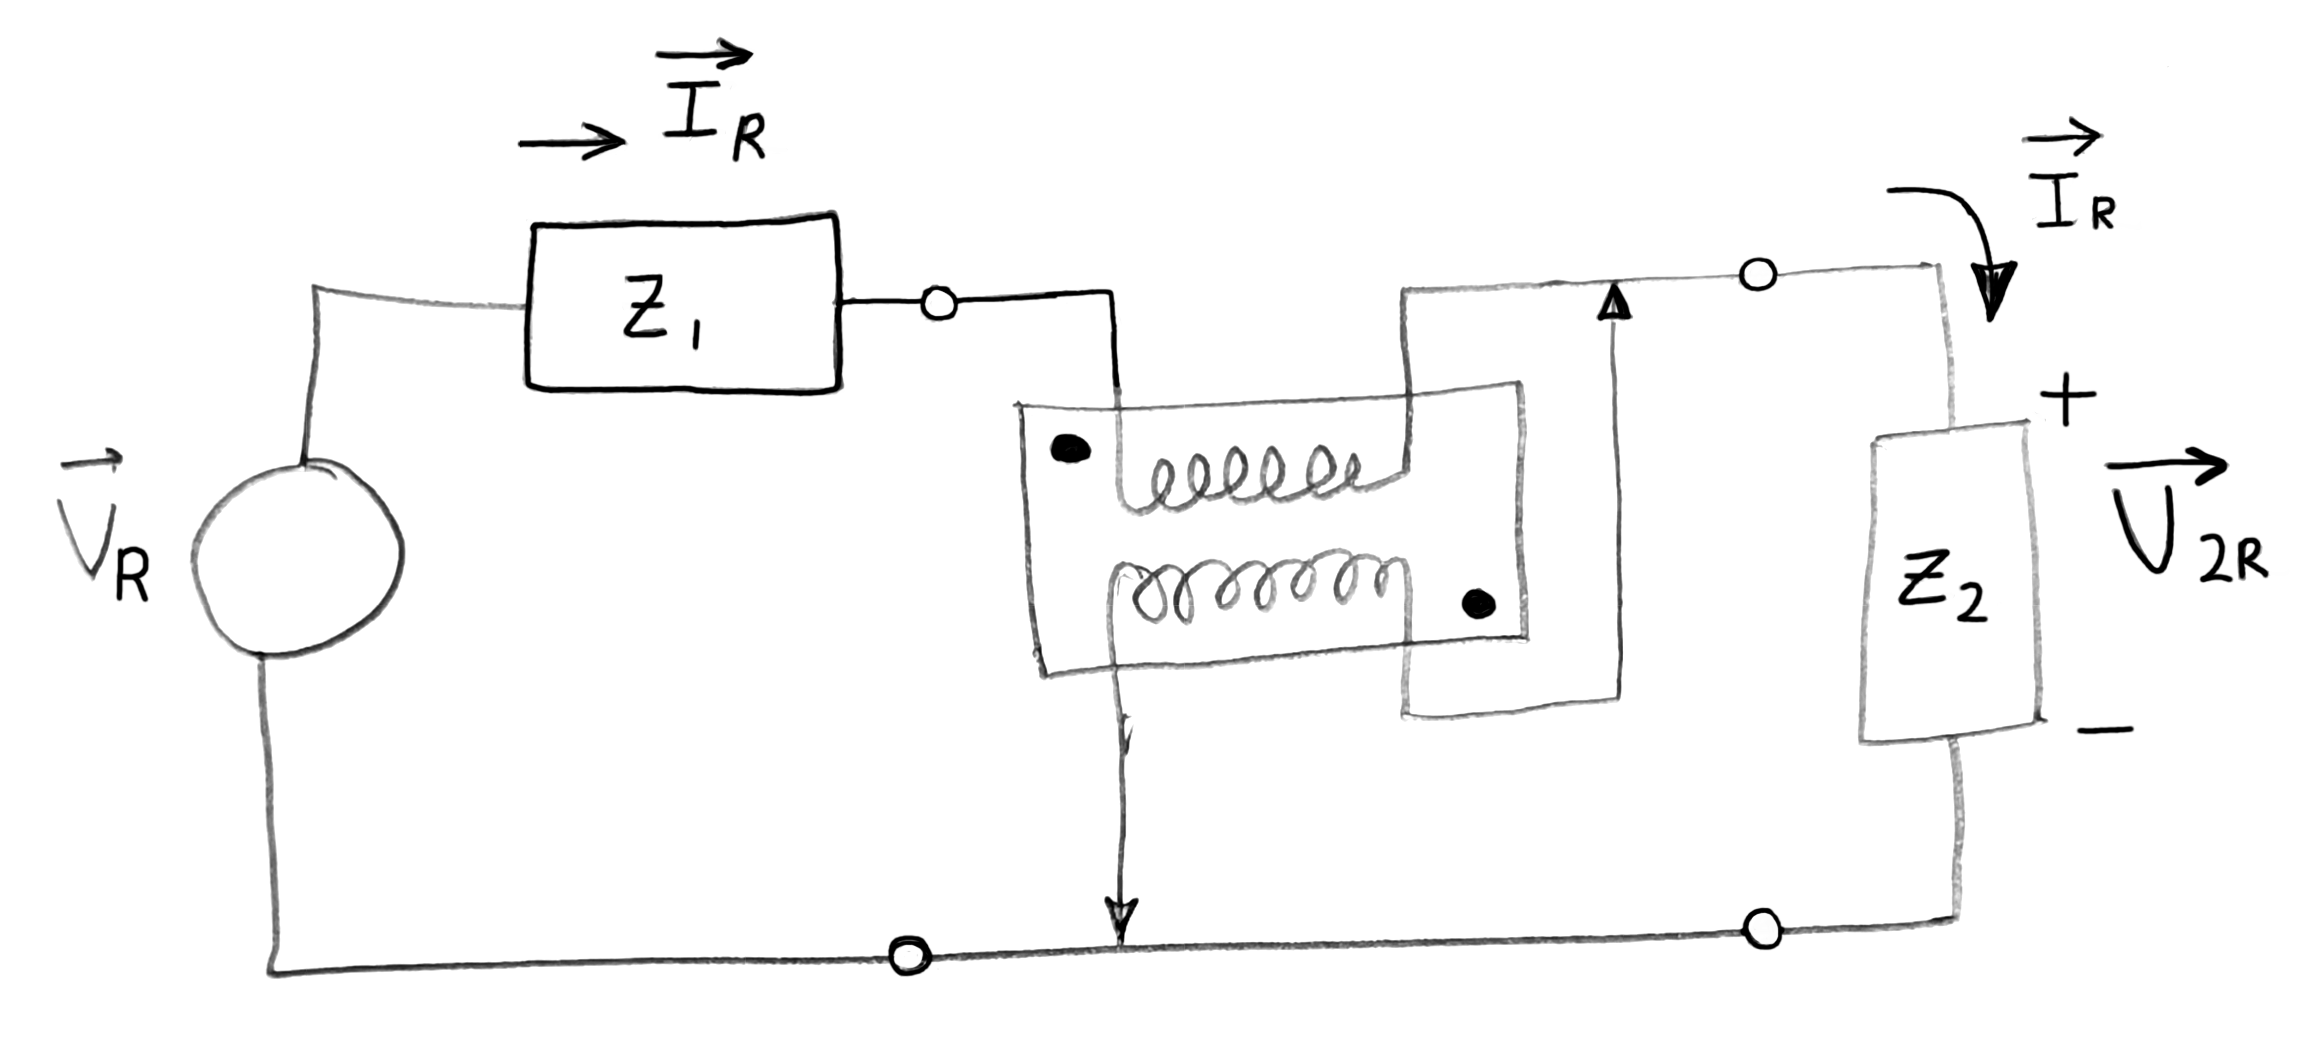
\includegraphics[width=125mm]{figsChapt03/GD42554.png}



We model a power plant and distribution system as a phasor Thevenin equivalent
circuit (left), and then connect a power meter between it and the load impedance $Z_2$
(right).

\vspace{0.2in}
\paragraph{Question: What will meter read?}

\paragraph{Solution:}
\[
\vec{I}_R = \frac{\vec{V}_R}{Z_1 + Z_2} \quad\quad\quad |\vec{I}_R| = \frac{|\vec{V}_R|}{| {Z}_1 +  {Z}_2|}
\]

Ignoring the ideal meter and using the voltage divider equation, we have

\hspace {1.75in} 1)
\[
\vec{V}_{2R} = \vec{I}_R Z_2 = \vec V_R \frac{Z_2}{(Z_1 + Z_2)}
\]

\[
S_{\text{Meter}} = \vec{I}_R\vec{V}_{2R}^*
\]
and also,

\[
P_{AV-Meter} = \mathrm{Re} \{S_{Meter}\} = |\vec I_R||\vec V_{2R}|\cos(\angle Z_2)
\]
We have


\hspace {1.75in} 2)
\[
\vec I_R = \frac {\vec V_{R}} {(Z_1+Z_2)}
\]
substituting,
\[
P_{AV-Meter} = \left |   \frac {\vec V_{R}}   {(Z_1+Z_2)}   \right |
\left | \vec V_R \frac{Z_2}{(Z_1 + Z_2)} \right | \cos(\angle Z_2)
\]
\[
= \frac{|\vec{V}_R| |\vec{V}_R| |Z_2|}
       {|(Z_1 + Z_2)|^2} \cos \angle Z_2
\]

\[\boxed{
P_{AV-Meter} = \frac{|\vec{V}_R|^2 |Z_2|}
                    {|(Z_1 + Z_2)|^2} \cos \angle Z_2
}
\]
(which will be the speed of the wheel inside the meter.)

\end{Example}










